
The following chapter describes the analysis with two same sign \hadtau and two jets performed with 8\tev data. After a brief description of the data and Monte Carlo samples, details follow on the selection used following the strategy suggested in Chapter \ref{sec:VBFSUSY}. The next section motivates and describes the data-driven background estimation technique used for treating QCD background events where two jets get mis-reconstructed as \hadtau and pass the event selection. Details on the validation method and systematic uncertainties are given in le last two sections.

\section {Data sample and trigger paths}

The analysis is performed using data collected with the CMS detector
in proton-proton collisions at a centre of mass energy of \CM = 8\tev at the LHC. The data samples correspond to an integrated luminosity of \lumiOld. 

The first analysis concept was relying on the usage of a VBF-based trigger for online selection. By doing its online selction  over the properties of the di-jet system

The original analysis design considered the usage of a VBF-based trigger. By doing the online selection over the properties of the hard jets coming from VBF processes, this trigger would a given a great freedom on the offline selection of the \hadtau properties and on \met.

However the available HLT trigger was seeded by \met L1 trigger that was fully efficient at roughly $\met > 250\gev$. Implementing such value in the offline event selection would have had a drastic impact on signal events statistics as previously shown on \autoref{fig:VBF_met_pttau}.

The other available trigger strategy was relying on the choice of a double-lepton trigger for each of the different search channel. In case of the \hadtau\hadtau channel the only unprescaled available alternative is the \texttt{HLT\_\-DoubleMedium\-IsoPFTau35\_\-Trk*\_\-eta2p1\_\-Prong1\_\-v*} trigger. This trigger is the least competitive among all the lepton trigger but is the one with the highest signal acceptance for the \hadtau channel. An efficiency study on the selected trigger is shown on \autoref{fig::trigger_turnon}.

 	\begin{figure}[tbh!]
	\centering
	\begin{tabular}{cc}
		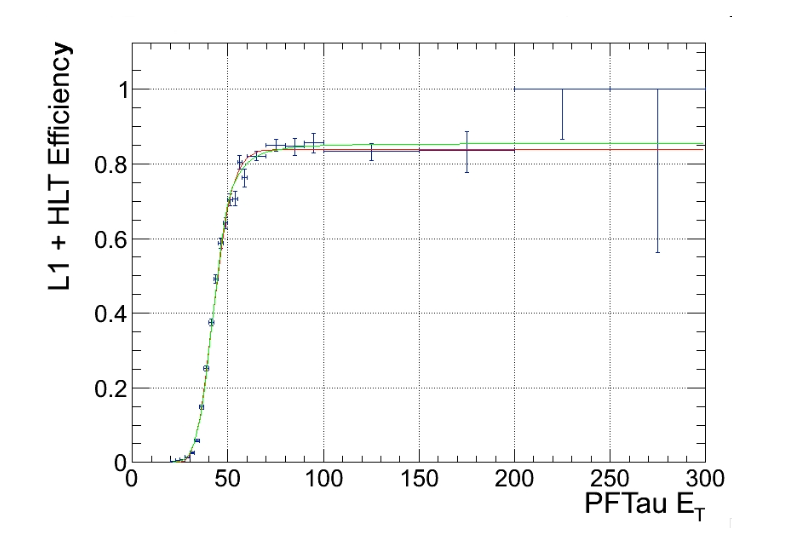
\includegraphics[width=0.75\textwidth]{analysis/pics/trigger_turnon.png}
	\end{tabular}
	\caption{Efficiency study on the \texttt{HLT\_\-DoubleMedium\-IsoPFTau35\_\-Trk*\_\-eta2p1\_\-Prong1\_\-v*} trigger versus the \hadtau transverse energy.The comparison of the fit curves given by the convolution of the step function with the Crystal Ball (in green) and the Gaussian (in red) is reported\cite{bib:dthesis:riccardoManzoni}.}
	\label{fig::trigger_turnon}
\end{figure}

\section{Signal and background samples}

%TODO you need to explain more precisely where MC is used: signal prediction, *part* of the bkg prediction, optimization, design of QCD background prediction

%TODO you use “normalize” for 2 different things. Rephrase to make clear  - that you *normalize* the MC yields to the integrated luminosity of the data (quote number) - *by using* cross sections predicted with …  

All the background yields, except for QCD, are taken from simulation. Simulated samples of signal and background events are generated using Monte Carlo event generators.

The signal event samples are generated with the \texttt{MadGraph v5.1.5} program \cite{Alwall:2011uj}, considering pair production of gauginos with two associated partons. The signal events are generated requiring a pseudorapidity gap $|\deltaeta| > 4.2$ between the two partons, with $\pt > 25\gev$ for each parton. Signal cross sections are calculated at leading order using the MadGraph generator. The range of signal cross sections is $50^{-1}$ fb for \charginopm = \neutralinotwo masses of 100, 200 and 300\gev.

Background event samples with a Higgs boson produced through VBF processes, and single top are generated with the \texttt{POWHEG v1.0r1380} program \cite{Frixione:2007vw}. 
The \texttt{MadGraph v5.1.3} generator is used to describe Z+jets, W+jets, tt, di-boson, and VBF Z boson production. The Monte Carlo background and signal yields are normalized to the integrated luminosity of the data. 
The \ttbar background is normalized to the next-to-next-to-leading-logarithm level using the calculations presented in references \cite{Czakon:2013goa,Melnikov:2006kv}. 
The Z+jets and W+jets processes are normalized to next-to-next-to-leading-order using the results from the \texttt{FEWZ v2.1} \cite{Gavin:2010az} generator. 
The di-boson background processes are normalized to next-to-leading-order using the \texttt{MCFM v5.8} \cite{Campbell:2010ff} generator, while the VBF Z boson events are normalized to next-to-leading order using the \texttt{VBFNLO v2.6} \cite{Arnold:2008rz,Arnold:2011wj}program. 
The single-top and VBF Higgs boson background yields are taken from the \texttt{POWHEG} program, where the next-to-leading order effects are incorporated.

All Monte Carlo samples incorporate the \texttt{CTEQ6L1} \cite{Pumplin:2002vw} or \texttt{CTEQ6M} \cite{Nadolsky:2008zw} parton distribution functions (PDF). The corresponding evaluation of uncertainties in the signal cross sections is discussed in Section \ref{sec:systematics}. The \texttt{POWHEG} and \texttt{MadGraph} generators are interfaced with the \texttt{PYTHIA v6.4.22} \cite{Sjostrand:2006za} program, which is used in the mathing between the matrix elements and the parton shower, and the hadronization processes. 


The decays of $\tau$ leptons are simulated using the \texttt{tauola (27.1215)} \cite{Davidson:2010rw} program. The background samples are processed with a detailed simulation of the CMS apparatus using the \texttt{Geant4} package \cite{Agostinelli:2002hh}, while the response for signal samples is modeled with the CMS fast simulation program \cite{Abdullin:2011zz}. For the signal acceptance and \mjj shapes based on the fast simulation, the differences with respect to the \texttt{Geant4}-based results are found to be small ($< 5\%$). Corrections are applied to account for the differences. 

For all Monte Carlo samples, multiple proton-proton interactions are superimposed on the primary collision process, and events are reweighted such that the distribution of reconstructed collision vertices matches that in data. The distribution of the number of pileup interactions per event has a mean of 21 and a root-mean-square of 5.5. 

For all datasets, a common \texttt{Physics Analysis Toolkit} (\texttt{PAT}) \cite{Adam:2010zza} sequence has been used to generate samples in PAT format, then further reduced them in size with the ntuple producer \cite{bib:thentuplemaker}.

%TODO how is the trigger modeled in MC? you use the same reconstruction software on MC as on data? 

%TODO (LOW PRIORITY) geant4 is not the full story: electronics and propagation of light through material is emulated (digitization step)(check recent CMS papers)

\section{Event Selection}
\label{sec:eventselection}

%TODO one topic per paragraph

%TODO read it again and try to make your text easier to understand for a reader that is less familiar with LHC analyses

As mentioned in Section \ref{section::search_strategy} the di-\hadtau channel's main background contribution comes from QCD multijetevents, with a rate several orders of magnitude larger than the rate of other background contributions. Hence this search channel, more than any of the other lepton channels, relies on the efficient background rejection. Fortunately, the VBF and \met selections provide the required background suppression.

All the collision data events passing the requirements of the triggers shown in Table \ref{table:triggerdefinition} are considered for offline analysis. 

As previously introduced in Section \ref{section::search_strategy}, the event selection criteria is divided in two distinct parts: the central part, which takes into account the LSP and the decay products of the multiple \hadtau, and the VBF part, which cuts on the kinematic properties of the jets coming from a VBF process. 

The main differences with the other VBF SUSY searches with final states including light leptons, are the substantially tighter \hadtau requirements targeting at the suppression of QCD jet background and the looser missing transverse energy (\met) requirement, to recover some of the signal acceptance lost due to the larger discriminator based on isolation $\hadtau$ \pt thresholds needed to stay efficient with respect to the trigger. 

There are some differences this analysis has with the other existing VBF searches with final states to light leptons. The most important ones are the substantially tighter requirements on the \hadtau isolation and \pt, which allows a good QCD background suppression while remaining efficient with the trigger online requirements. However those requirements leads also to a reduction in the signal acceptance, for that reason a looser \met cut is introduced.

The selected events are required to have at least two \hadtau candidates as defined in Section \ref{subsec::objsel_tau}. The reconstruction of more than two \hadtau is constrained by the trigger. The like sign \hadtau candidates with the highest \pt and separated from each other by a minimum \deltar = 0.3 are then chosen to form a di-\hadtau candidate. 
Further, to reduce top pair contamination the event is required not to have any jet identified as a b--quark jet by the b--tagging algorithms using the {\textit combined secondary vertex loose} (CSVL) working point. 

Only jets with \pt $\ge 30\gev$ and separated from the taus in the di--\hadtau pairs by $\Delta R \ge 0.3$ are searched for b--tags. The \pt cut of 30\gev on b-jets (a looser veto requirement than other analyses with light leptons) allows to be more efficient with respect to the signal since the higher \pt threshold on taus reduces the contamination of $t\overline{t}$ to a large extent. Further, the event is required to have at least 30\gev of \met in order to further reduce QCD contamination. All the selections described above is what will be referred to as \textit{central selections}.

Subsequently, the following event-wide requirements are imposed. The {\textit {VBF selections}} are imposed by requiring at least two jets as defined in Section \ref{subsec::objsel_jet}. Only jets separated from the leptons in the \hadtau\hadtau pair by $\deltar \ge 0.3$ are considered. All jet candidates passing the above requirements and having $\vert \Delta\eta \vert \ge 4.2$ and $\eta_{1}\cdot\eta_{2} < 0$ are combined to form di-jet candidates. The final and the most important of the requirement is an invariant mass of the di-jet candidate, denoted \mjj, above the threshold of 250\gev. In order to increase the event acceptance the analysis code algorithm takes into account every possible di-jet candidate combination and chooses the one that passes the VBF requirements and has the highest \mjj. 

For better visualization and understanding all the selection criteria are summarized the following way:

%TODO (LOW priority) it’s more elegant to have this in a table instead of a bullet list.

\begin{itemize}
	\item \textbf{VBF selection}
	\begin{itemize}
		\item at least two jets with $p_{T}^{jet}\geq30~$\gev, $|\eta_{jet}|\leq5$ and loose jetID
		\item $|\Delta\eta(jet,jet)| > 4.2$
		\item $sign(\eta^{jet 1}\cdot\eta^{jet 2})==-1$
		\item $\mjj>250~$\gev
	\end{itemize}
	\item \textbf{Central selection}
	\begin{itemize}
		\item Trigger: \texttt{HLT\_DoubleMediumIsoPFTau35\_Trk*\_eta2p1\_Prong1\_v*}
		\item two one-prong hadronically decaying $\tau$ with $\pt\geq45~$\gev 
		\item $\met > $ 30\gev
		\item $\Delta R(jet,\tau)\geq0.3$
		\item b-tag veto
	\end{itemize}
\end{itemize}

%todo (LOW PRIORITY) you need a cutflow table here, and a discussion about how event yields for data and MC samples reduces with cuts.

\clearpage



\section {Data-Driven QCD background determination} \label{sec:bgestimation}

%TODO improve flow of information, e.g.
%TODO 1. short introduction to the concept
%TODO 2. definition of control regions ( table with event yields)
%TODO 3. assumptions
%TODO 4. the actual method

The QCD background contribution for the like-sign di-\hadtau channel is done using a ABCD data-driven approach. This method consist in dividing the analyzed data in different exclusive regions, defined by two variables. The first variable is the \hadtau isolation discriminator used in the object reconstruction, namely:
 	
 	%TODO don’t use these funny names here: just use “tight”, “loose” and “medium”, introduced in the object definition, with a reference such that the really interested can find back what you exactly mean. and you have the appendix anyway.
 	
 	\begin{enumerate}
 		\item Tight (T) isolated $\hadtau$ for \texttt{byTight\-Isolation\-MVA3\-newDMwLT};
 		\item Medium (M) isolated $\hadtau$ for \texttt{byMedium\-Isolation\-MVA3\-newDMwLT} but failed \texttt{byTight\-Isolation\-MVA3\-newDMwLT};
 		\item Loose (L) isolated $\hadtau$  for \texttt{byLoose\-Isolation\-MVA3\-newDMwLT} but failed \texttt{byTight\-Isolation\-MVA3\-newDMwLT} and \texttt{byMedium\-Isolation\-MVA3\-newDMwLT}.
 	\end{enumerate}
 	
Each event with a successfully reconstructed LS di-$\hadtau$ pair falls into a exclusive isolation region as shows on Figure \ref{fig:tauisoregions}:
 	
 	\begin{itemize}
 		\item 2T or signal region (SR) consisting of two tight isolated $\hadtau$;
 		\item One Tight (1T) isolated $\hadtau$ region consisting of one tight isolated $\hadtau$ and an additional medium or loose isolated $\hadtau$;
 		\item  Anti Tight (AT) isolation region consisting of at least one medium isolated $\hadtau$ and an additional medium or loose isolated $\hadtau$;
 		\item  Anti Medium (AM) isolation region consisting of two loose isolated $\hadtau$.
 	\end{itemize}
 
 	\begin{figure}[tbh!]
 		\centering
 		\begin{tabular}{cc}
 			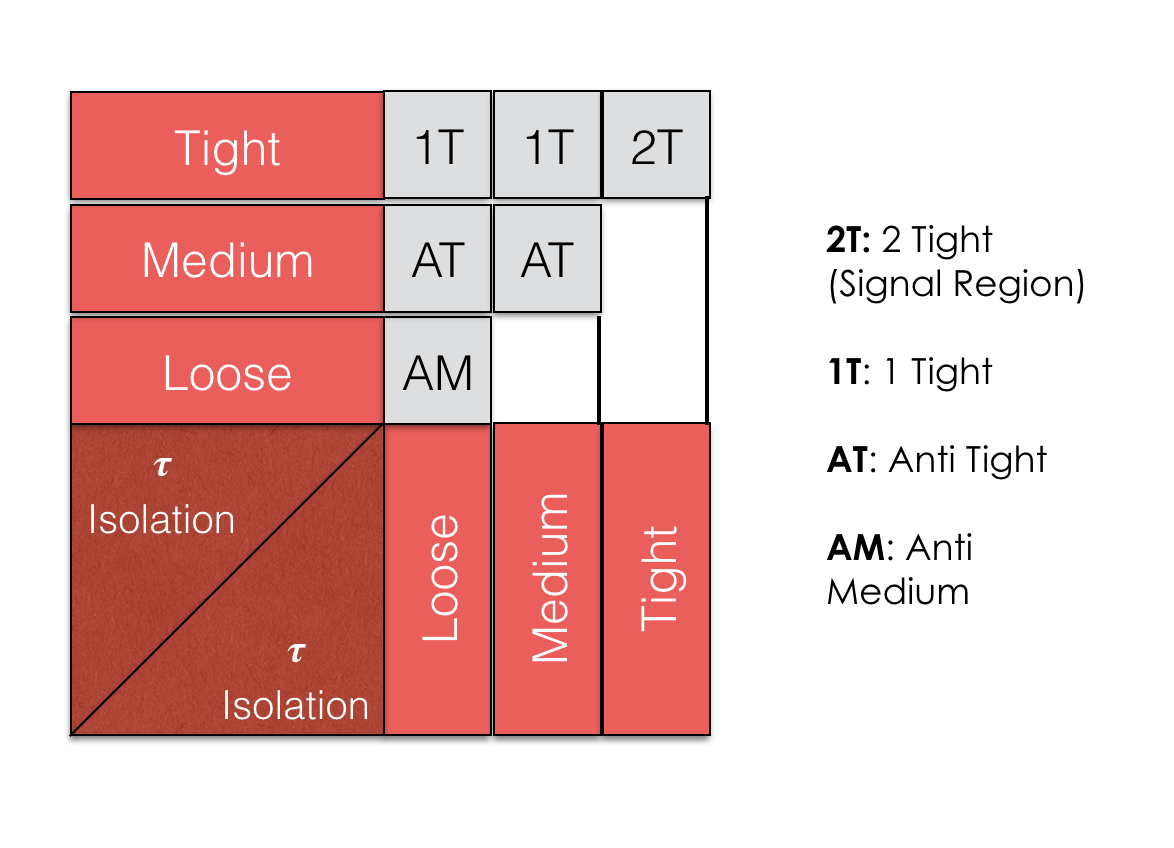
\includegraphics[width=0.75\textwidth]{PLOTS/diTauHadLSotherPlots/tauisoregions.png}
 		\end{tabular}
 		\caption{Definitions of the exclusive isolation region depending on the isolation of each of the $\hadtau$ where SR is Signal Region consisting of two tight isolated $\hadtau$, 1T is One Tight isolated Tau region consisting of one tight isolated $\hadtau$ and an additional medium or loose isolated $\hadtau$, AT is Anti Tight isolation region consisting of at least one medium isolated $\hadtau$ and an additional medium or loose isolated $\hadtau$,  AM is Anti Medium isolation region consisting of two loose isolated $\hadtau$}
 		\label{fig:tauisoregions}
 	\end{figure}
 
The second dimension of exclusivity is based on the VBF cuts described in \ref{sec:eventselection}. The regions are defined the following way:
	
	\begin{enumerate}
		\item VBF region: consisting of all the events that passed all VBF cuts previously mentioned in \autoref{sec:eventselection};
		\item VBF inverted region: consisting of all the events that at least fails one of the VBF cuts previously mentioned.
	\end{enumerate} 

Using these definitions one signal region (SR) and seven control regions (CR) are defined as shown in Figure \ref{fig:crs}. The SR falls into the region defined by two tight isolated $\hadtau$ and all the VBF cuts applied, close to it the control region two (CR2) features the same \hadtau isolation requirements but inverted VBF selection requirement. The remaining control regions are defined as CR3 (One Tight isolation region), CR5  (Anti Tight isolation region) and CR7 (Anti Medium isolation region) followed by their corresponding VBF-inverted control regions CR4, CR6, CR8. An overview of the defined SR and CRs is shown on \autoref{fig:crs}.

\begin{figure}[tbh!]
	\centering
	\begin{tabular}{cc}
		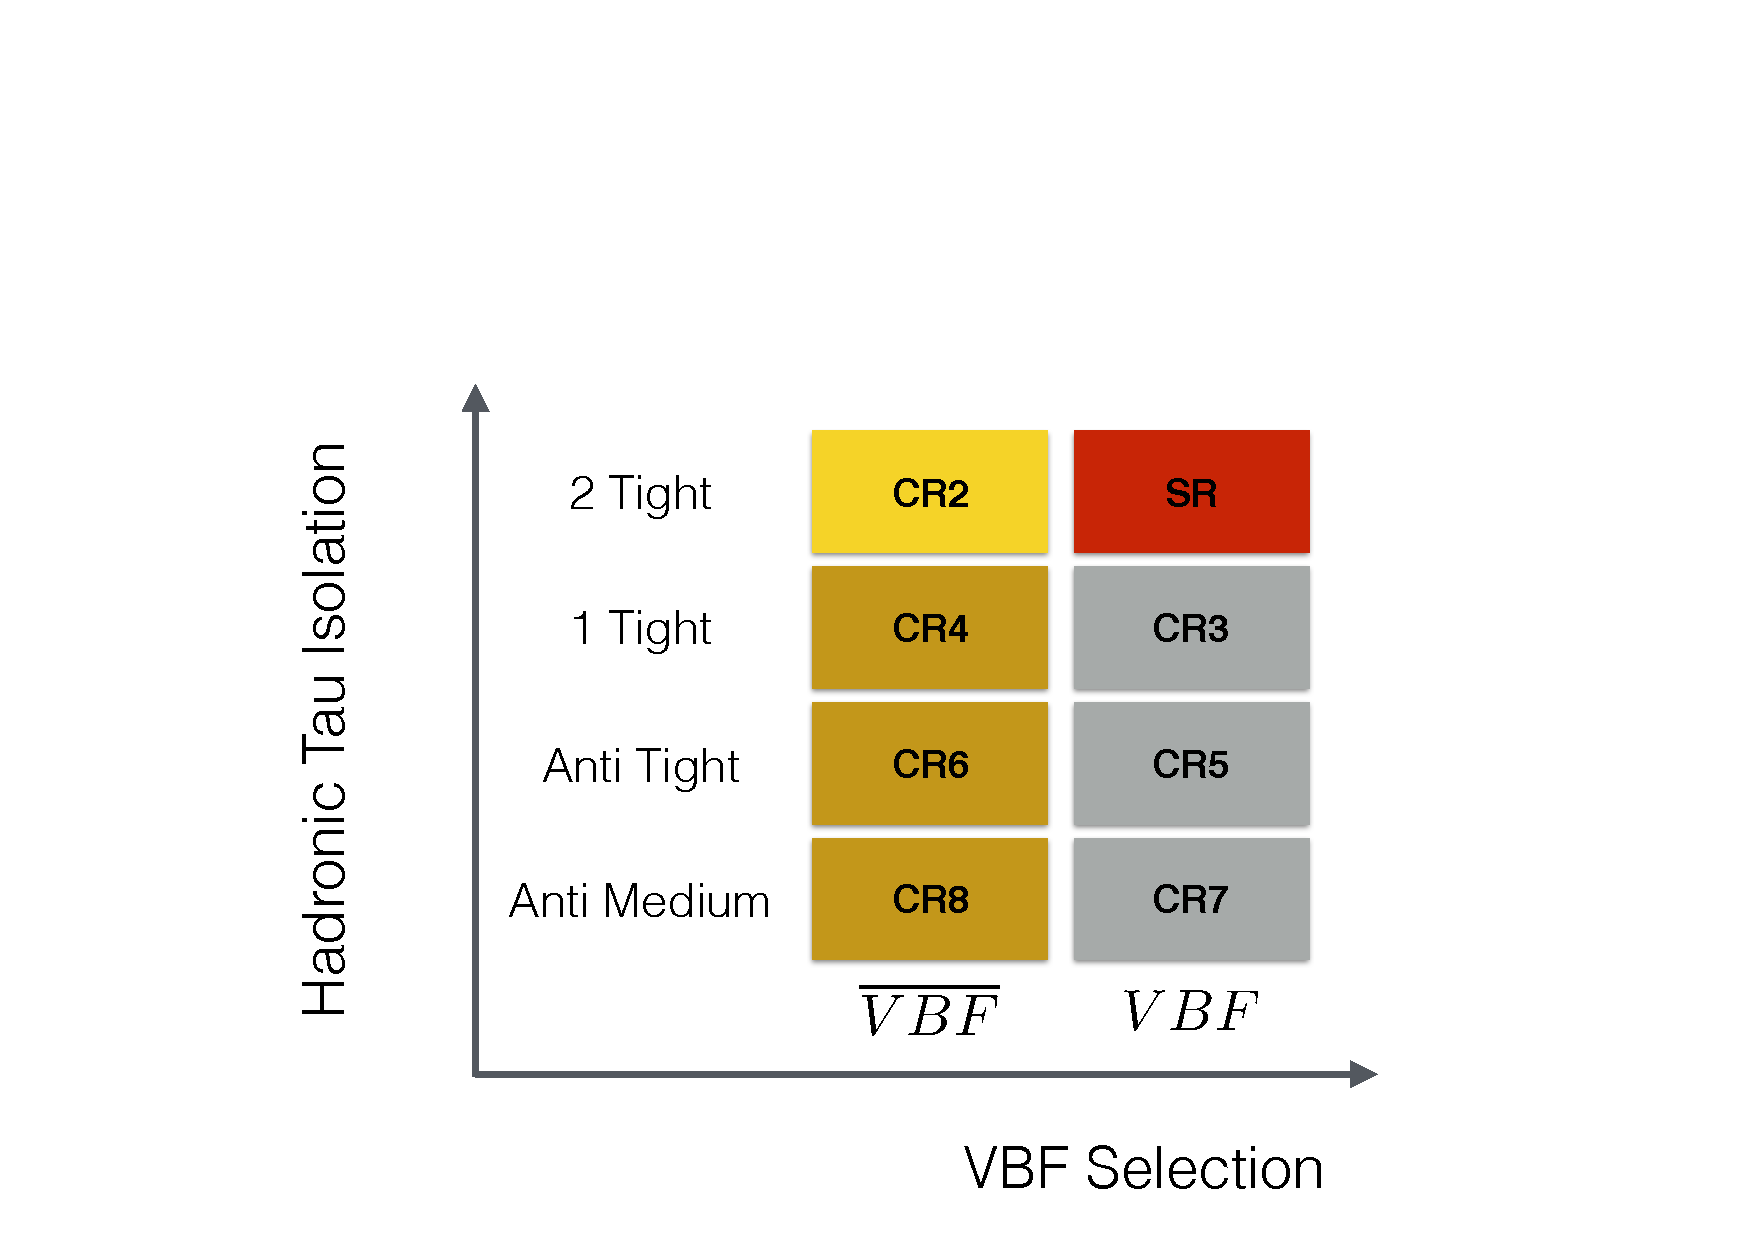
\includegraphics[width=0.75\textwidth]{PLOTS/diTauHadLSotherPlots/controlregions.pdf}
	\end{tabular}
	\caption{Definition of Signal and Control Regions using different $\hadtau$ isolation criteria and VBF selection.}
	\label{fig:crs}
\end{figure}

The estimation of the events in the signal region is equivalent to the classic ABCD method consisting in counting the number of events in CR2 and multiplying it with a proper conversion factor. This estimation method has been developed under the following assumptions:

\begin{itemize}
	\item The VBF selection efficiency is independent from any trigger efficiency concerning $\hadtau$ isolation such that each contribution to the numerator and denominator cancels out;
	\item The VBF selection efficiency is also independent from any \met cut applied in order to reduce QCD background contributions. 
\end{itemize}

The predicted number of QCD events in the signal region $N^{QCD}_{SR}$ is defined as:

\begin{equation}
N^{QCD}_{SR} = \left( N^{DATA}_{CR2} - N^{\overline{QCD} BG}_{CR2} \right) * \left[ \frac{\epsilon^{QCD}_{VBF}}{1 - \epsilon^{QCD}_{VBF}} \right]
\label{eq:qcdbgpred}
\end{equation}

where $N^{DATA}_{CR2}$ is the number of data events in CR2, $N^{\overline{QCD} BG}_{CR2}$ is the number of all non-QCD Monte Carlo samples events in CR2 and $\epsilon^{QCD}_{VBF}$ is the efficiency of VBF cuts in a lower \hadtau isolation region. 

The $\epsilon^{QCD}_{VBF}$ for each of the different \hadtau isolation region is with the following equation.

\begin{equation}
\epsilon^{QCD}_{VBF} = \frac {N^{DATA}_{VBF CR} - N^{\overline{QCD} BG}_{VBFCR}}{\left( N^{DATA}_{VBFCR} - N^{\overline{QCD} BG}_{VBFCR} \right) + \left( N^{DATA}_{\overline{VBF}CR} - N^{\overline{QCD} BG}_{\overline{VBF}CR} \right) }
\label{eq:vbfeff}
\end{equation}

where $N^{DATA}_{VBF CR}$ is the number of the events in data for a given $ \tau $ isolation region and VBF region, $N^{\overline{QCD} BG}_{VBFCR}$ is the number of all non-QCD Monte Carlo events for a given $ \tau $ isolation region and VBF region, $N^{DATA}_{\overline{VBF}CR}$ is the number of events in data in the same isolation Control Region but inverted VBF region and$N^{\overline{QCD} BG}_{\overline{VBF}CR}$ is the number of all non-QCD Monte Carlo events for a given $ \tau $ isolation region but inverted VBF region.

Using the events in the defined control regions coming from \autoref{table:CReventcount} as input for \autoref{eq:qcdbgpred} and \autoref{eq:vbfeff} is possible to determine three independent predictions for the QCD background contribution, one for each pair of tau isolation control regions below the two-tight isolation region. \autoref{table:CReventcount} shows the event counting for all the control regions previously defined for data and all Monte Carlo samples. All the numbers except the ones coming from the QCD sample are used as input for the QCD background estimation method. All the statistical uncertainties are propagated accordingly.  For each of the three different $\tau$ isolation regions out of the signal region (1T, AT, AM) an independent measurements of $\epsilon^{QCD}_{VBF}$  and prediction for $N^{QCD}_{SR}$ is made. A validation of the data-driven background prediction is performed  using a simulation-driven approach. Details and results on this methods are given in \autoref{QCD_bg_pred_validation}.

Three sources of systematic uncertainty has been considered in the estimation of the QCD contamination in the signal region shown in \autoref{eq:qcdbgpred}. The first source comes from the uncertainty over the generated Monte Carlo samples used in the analysis. The two remaining ones come from the assumptions about the stability of the $\epsilon^{QCD}_{VBF}$, made when defining the data-driven method, one in regard to the relaxation of the tau-identification and the other in regard to a loosening of the \met cut, since the $\epsilon^{QCD}_{VBF}$ is calculated in CRs where no \met cut is applied.

The uncertainty given by a systematic error in the Monte Carlo simulation is estimated by checking the maximal variation over $\epsilon^{QCD}_{VBF}$ and $N^{QCD}_{SR}$ after scaling non-QCD contributions by $\pm50~\%$. 

The remaining systematics uncertainties on the $\epsilon^{QCD}_{VBF}$ are estimated using a simulation-based approach as described in \autoref{dihad:subsec:stability}.

\begin{sidewaystable}
	\centering
	\begin{tabular}{| l | c | c | c | c | c |}
		\hline\hline
		Sample       &Events (CR2)     &Events (CR3)  &Events (CR4)  &Events (CR5)     &Events (CR6)  \\ [0.5ex] \hline
		Data    &$ 109$    &$ 39$   &$ 737$  &$ 22$    &$ 312$  \\
		Drell-Yan    &$ 1.3\pm1$    &$ 0.042\pm0.0077$     &$ 0.65\pm0.045$  &$ 0.002\pm0.00076$    &$ 0.029\pm0.0037$    \\
		VV     &$ 0.7\pm0.09$    &$ 0.035\pm0.017$    &$ 0.6\pm0.1$   &$ 0.0031\pm0.001$    &$ 0.045\pm0.015$   \\
		W+Jets     &$ 6.6\pm0.17$    &$ 0.83\pm0.055$    &$ 10\pm0.2$  &$ 0.081\pm0.0096$    &$ 0.89\pm0.034$      \\
		Single t     &$ 0.25\pm0.017$    &$ 0.057\pm0.008$   &$ 0.47\pm0.02$   &$ 0.011\pm0.00076$   &$ 0.1\pm0.0028$     \\
		\ttbar    &$ 1.4\pm0.051$    &$ 0.19\pm0.013$   &$ 2.5\pm0.059$   &$ 0.04\pm0.0024$    &$ 0.52\pm0.0095$      \\
		Higgs     &$ 0.012\pm0.0048$    &$ 0.0029\pm0.0023$   &$ 0.012\pm0.0044$   &$ 2.7\cdot 10^{-05}\pm1.1\cdot	10^{-05}$    &$ 0.00018\pm2.2\cdot 10^{-05}$   \\
		QCD     &$ 54\pm1.2$    &$ 47\pm1.9$   &$ 3.4\cdot10^{+02}\pm4$  &$ 19\pm0.68$    &$ 1.4\cdot 10^{+02}\pm1.6$    \\
		[0.5ex] \hline
		Total $\overline{QCD}$ Monte Carlo    &$ 10\pm1$    &$ 1.2\pm0.06$   &$ 15\pm0.24$ &$ 0.14\pm0.01$    &$ 1.6\pm0.038$   \\
		\hline\hline
	\end{tabular}
\caption{Number on events in all the defined control regions for data and all Monte Carlo samples used for the estimation of $N^{QCD}_{SR}$}
\begin{tabular}{| l | c | c | }
			\hline\hline
Sample      &Events (CR7)     &Events (CR8)  \\ [0.5ex] \hline
Data     &$ 17$    &$ 184 $  \\
Drell-Yan    &$ 0.0012\pm0.00057$    &$ 0.013\pm0.0021 $  \\
VV   &$ 0.0011\pm0.00014$    &$ 0.033\pm0.016 $  \\
W+Jets    &$ 0.036\pm0.0051$    &$ 0.35\pm0.015 $  \\
Single t   &$ 0.0061\pm0.00045$    &$ 0.058\pm0.00087 $  \\
\ttbar  &$ 0.022\pm0.00079$    &$ 0.32\pm0.0054 $  \\
Higgs  &$ 4.9\cdot10^{-06}\pm2.3\cdot 10^{-06}$    &$ 5.7\cdot 10^{-05}\pm1\cdot 10^{-05} $  \\
QCD  &$ 15\pm0.81$    &$ 1.1\cdot 10^{+02}\pm1.7 $  \\
\hline
Total nonQCD Monte Carlo  &$ 0.067\pm0.0053$    &$ 0.77\pm0.023 $  \\
\hline\hline
\end{tabular}
\label{table:CReventcount}
\end{sidewaystable}

\begin{table}[ht]
	\centering{
		\tabcolsep=0.05cm
		\begin{tabular}{| l | c | c | c |}
			\hline\hline
			Variable     &One Tight region     &Anti-Tight region     &Anti-Medium  \\ [0.5ex] \hline
			$\epsilon^{QCD}_{VBF}$    &$ 0.05\pm0.008 $  &$ 0.066\pm0.014 $  &$ 0.085\pm0.02 $ \\
			$N^{QCD}_{SR}$    &$ 5.2\pm1 $  &$ 6.9\pm1.7 $  &$ 9.1\pm2.5 $ \\
			\hline\hline
		\end{tabular}
	}
	\caption{ Values for $\epsilon^{QCD}_{VBF}$ and $N^{QCD}_{SR}$ for different $ \tau $ isolation regions.}
	\label{table:VBFeffBKGprediction} % is used to refer this table in the text
\end{table}

\section{Validation of the Data Driven method }
\label{QCD_bg_pred_validation}

The data-driven background estimation method, as previously shown, offered a possibility to circumvent the scarce statistics of the simulated QCD samples. The results given in \autoref{section:results} can be backed by a simulation based approach which come with two main advantages. First, this it can confirm the assumption made for the data-driven method which states that all control regions and the signal region are indeed dominated by QCD events. Second, this approach can show that VBF efficiency $\epsilon^{QCD}_{VBF}$ defined in \autoref{eq:vbfeff} is independent, within the systematic uncertainty, with respect to a selection over \met or \hadtau transverse momentum. This section will give a brief description and results of this simulation based approach as presented in the PhD thesis of Denis Rathjens \cite{bib:phdthesis:denis}.

\subsection{The simulation-based method}
\label{dihad:subsec:eventweight}

A solution to the scarce statistics of the QCD sample in the signal region can be solved by taking all the events with at least four reconstructed jets and properly reweighting each one of them. This weight is a function of the probabilities that two of those four reconstructed jets will fake an \hadtau:

\begin{equation}
w^{TT}_{\text{event}} = \sum_{i=0}^{N}P(\text{iso}\mid \text{jet}_{i})\left(\sum_{j=0; j\neq i}^{N}P(\text{iso}\mid \text{jet}_{j})\left[\prod_{k=0; k\neq i,j}^{N}(1-P(\text{iso}\mid \text{jet}_{k}))\right]\right)
\end{equation}

where $P(\text{iso}\mid \text{jet})$ is the probability for a given jet to fake an \hadtau with a given isolation:

\begin{equation}
P(\text{iso}\mid \text{jet}_{i}) = P(\text{iso ID}\mid \text{jet}_{i}) \cdot P(\pt^{\hadtau(\text{fake})} > 45\gev\mid \text{jet}_{i}) \dot \epsilon^{\text{trigger}}(\text{ID})
\end{equation}

where $P(\text{iso ID}\mid \text{jet}_{i})$ is the probability for a given jet to fake a \hadtau with a given TauID selection besides the \pt requirement, $P(\pt^{\hadtau(\text{fake})} > 45\gev\mid \text{jet}_{i})$ is the probability for a given jet reconstructed as fake-\hadtau to pass the requirement of $\pt(\hadtau)> 45\gev$ and $\epsilon^{\text{trigger}}(\text{ID})$ is the efficiency of the trigger ,the one used in the analysis, in selecting events with at least four jets.

The most optimal way to represent $P(\text{iso ID}\mid \text{jet}_{i})$ is through a parametrization of the most significant jet variables. Closure studies done over different types of parametrization shows that the best parameters choice is the jet candidate \pt and the its charged hadron fraction $F_{q}$.

It is not granted that a jet ,with $\pt(\hadtau)> 45\gev$, which gets mis-reconstructed offline as \hadtau passes also the TauID \pt selection. Several are the reasons behind this effect. The most important one is that jets have energy corrections while \hadtaufake do not, which directly translates into slight deviations of the reconstructed object directions. It is possible to correct the \hadtau transverse momentum by a factor to match the \pt from the original jet. It is also important to correct the mass of the \hadtaufake by a factor which takes into account the difference in size of the reconstruction cone used for the jet and \hadtau objects.

The last of the corrections is the efficiency of the di-$\tau$ trigger in selecting events with two fake \hadtau , $\epsilon^{\text{trigger}}(\text{ID})$. This efficiency is derived for a single \hadtaufake from a study over W+jets events where one of the jets fakes an \hadtau.

This method, also called "dicing", is applied for QCD samples and W+jet samples, in the case where only one of the jets is reconstructed as \hadtaufake. 	\autoref{fig::CR2_controlplots1} and \autoref{fig::CR2_controlplots2} show a very good agreement between data and Monte Carlo for di-\hadtau and \met distributions in control region 2. All shown QCD distributions are scaled in order to exactly match the difference between the amount of data measured to the amount of non-QCD background events expected in the control region with the exception of the signal region where the scaling is done to the prediction of the ABCD method performed on data \cite{bib:phdthesis:denis}.


\begin{figure}[tbh!]
	\centering
	\begin{tabular}{cc}
		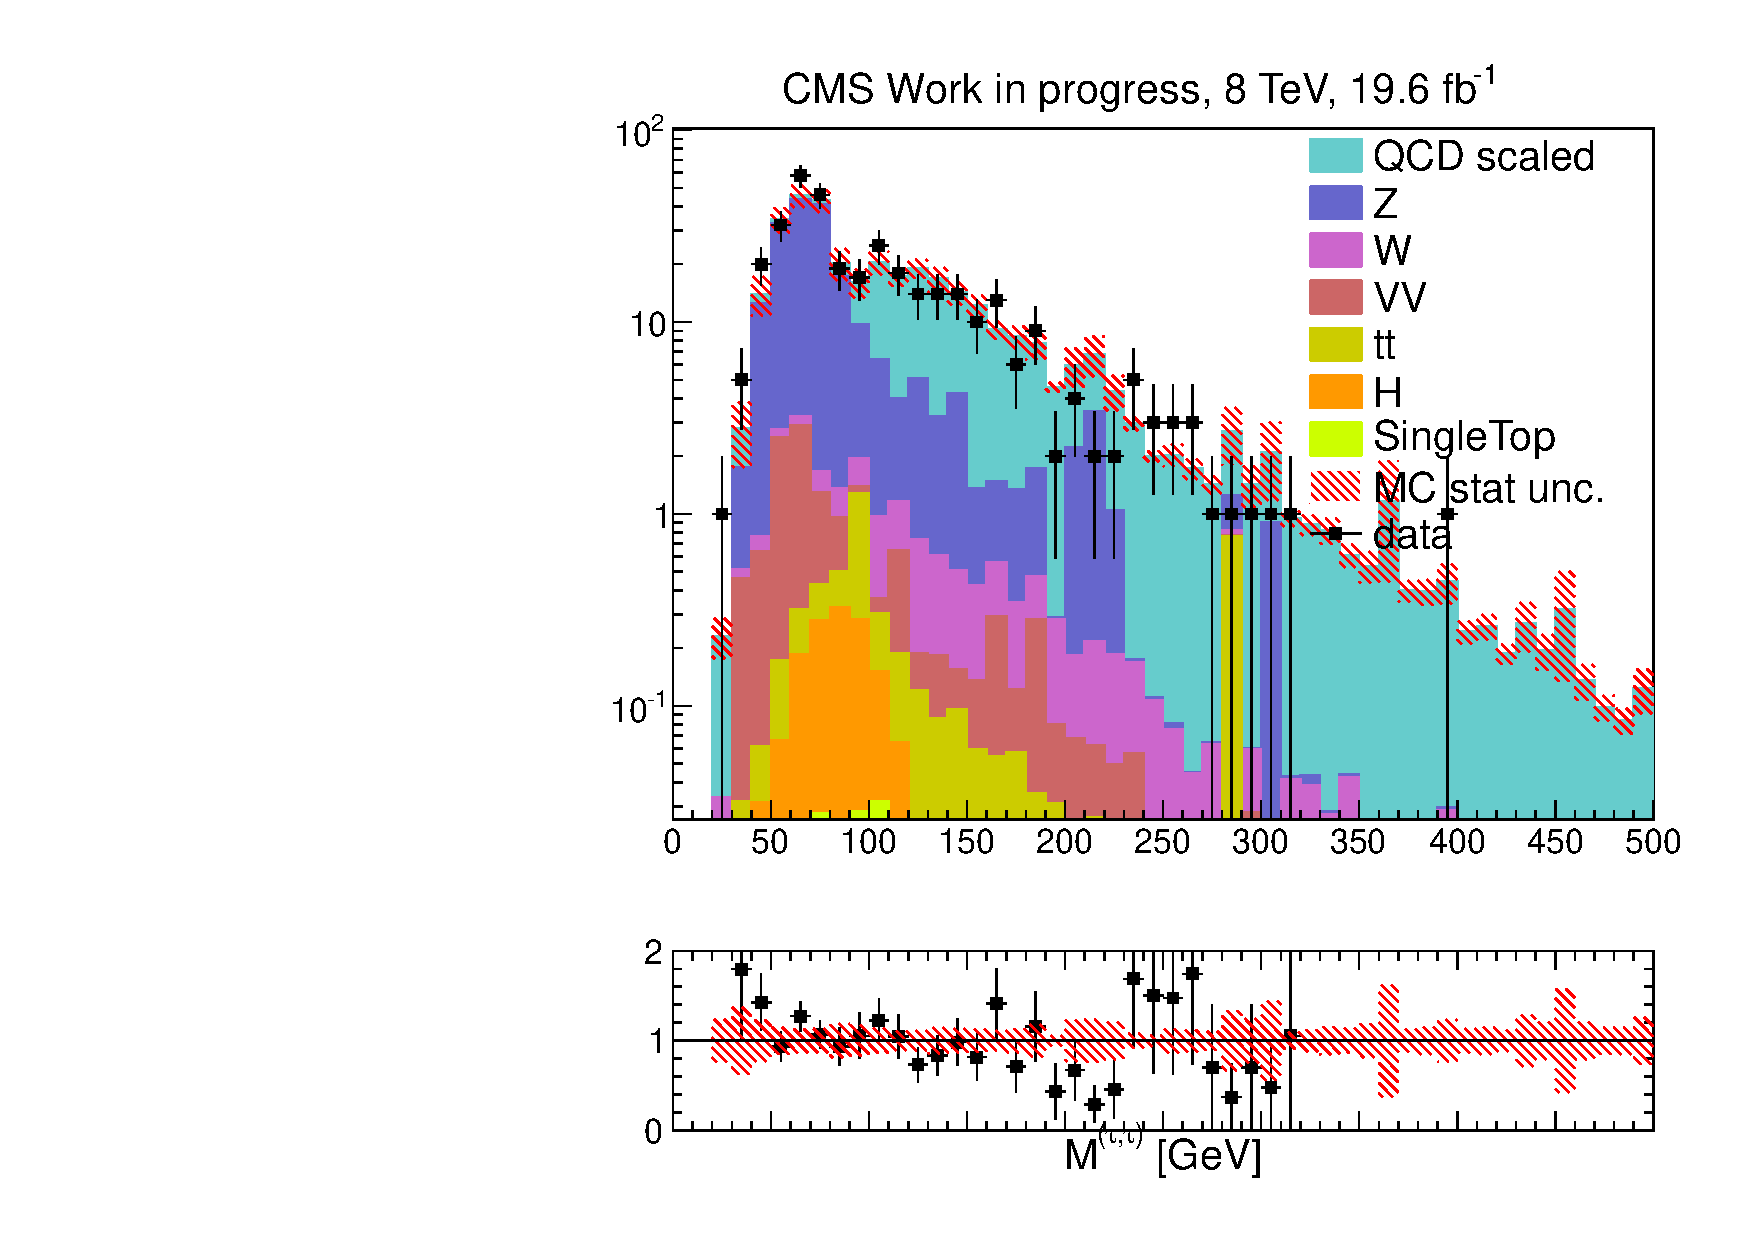
\includegraphics[width=0.45\textwidth]{PLOTS/diTauHadLSQCDPlots/AllMCdiced/OS_CR2/OS_Central_invertedVBF_2TightIso_CR2/h_ditauinvariantmass_log.pdf}
		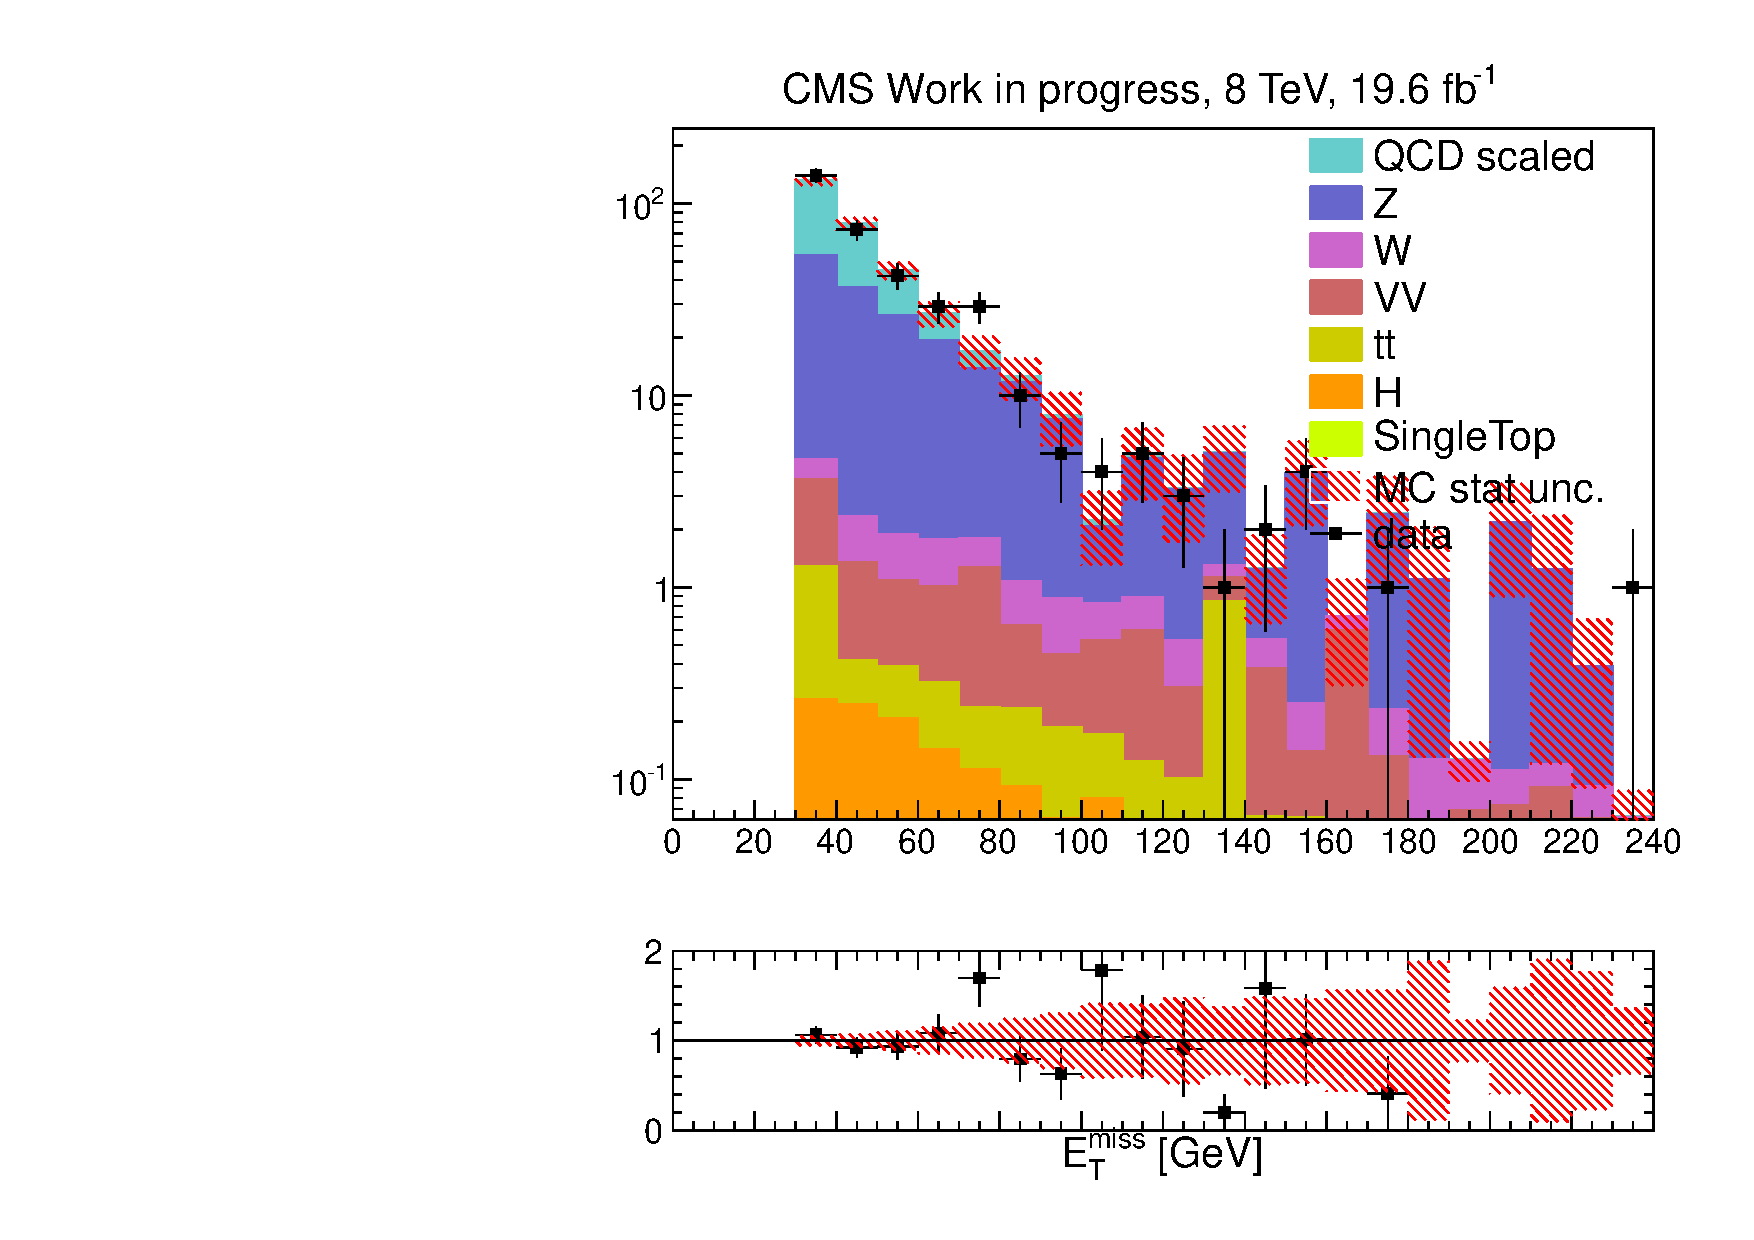
\includegraphics[width=0.45\textwidth]{PLOTS/diTauHadLSQCDPlots/AllMCdiced/OS_CR2/OS_Central_invertedVBF_2TightIso_CR2/h_met_log.pdf} 		
	\end{tabular}
	\caption{(Left) di-\hadtau invariant mass and (Right) \met distribution for control region 2.}
	\label{fig::CR2_controlplots1}
\end{figure}

\begin{figure}[tbh!]
	\centering
	\begin{tabular}{cc}
		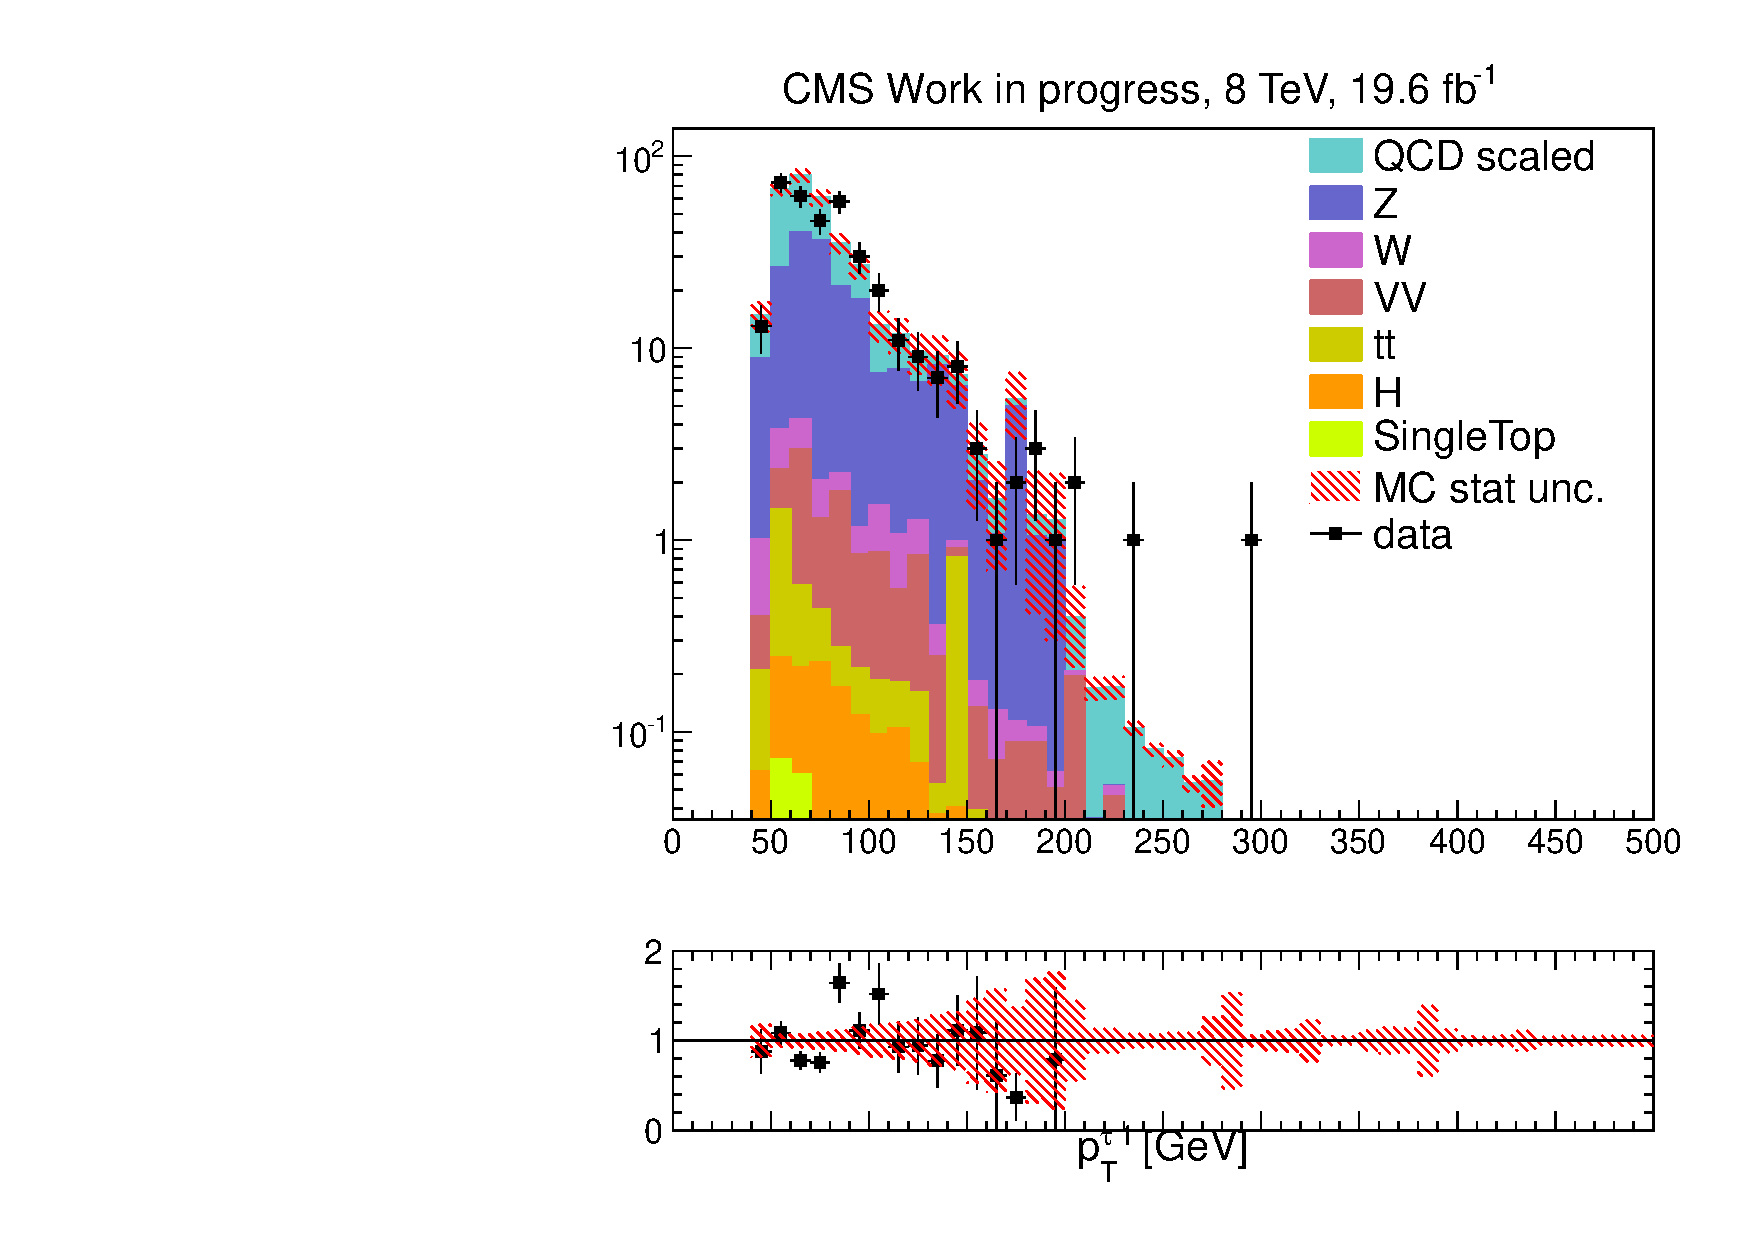
\includegraphics[width=0.45\textwidth]{PLOTS/diTauHadLSQCDPlots/AllMCdiced/OS_CR2/OS_Central_invertedVBF_2TightIso_CR2/h_tau1pt_log.pdf}
		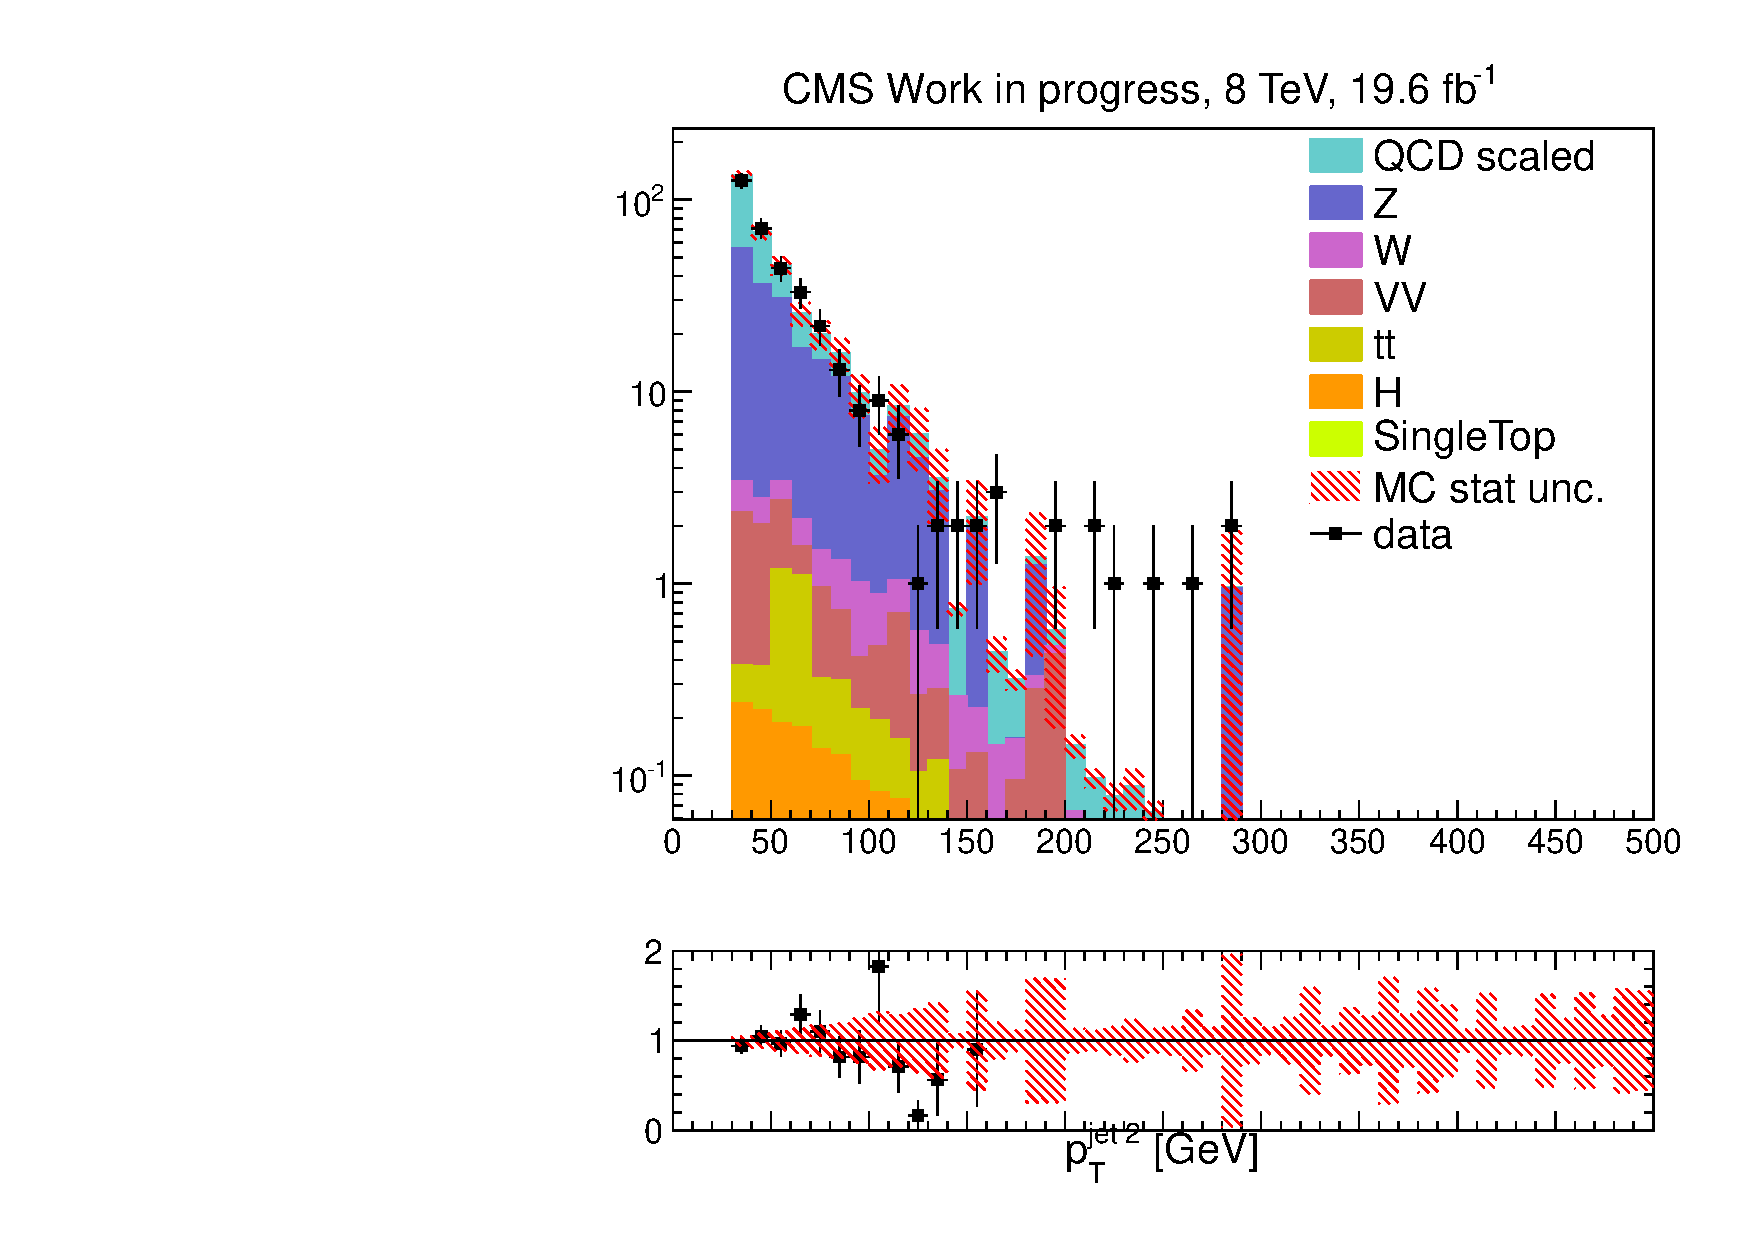
\includegraphics[width=0.45\textwidth]{PLOTS/diTauHadLSQCDPlots/AllMCdiced/OS_CR2/OS_Central_invertedVBF_2TightIso_CR2/h_jet2pt_log.pdf} 		
	\end{tabular}
	\caption{(Left) Leading \hadtau traverse momentum and (Right) next to leading jet transverse momentum for control region 2.}
	\label{fig::CR2_controlplots2}
\end{figure}

\subsection{$\epsilon^{VBF}$-stability with regard to $\tau_{h}$-isolation and $E_{T}^{miss}$-cuts}
\label{dihad:subsec:stability}

The efficiency of the VBF selection $\epsilon^{VBF}$ has been defined under the assumptions that is independent, within statistical uncertainty, from a selection over \met and \hadtau isolation.
 
 A study on the efficiency stability as function of the second leading \hadtau momentum is done over different tau isolation requirements as shown on \autoref{dihad:fig:vbeff_vs_tauiso}. The chosen \hadtau isolation selection is requiring two tight isolated \hadtau (TT) or one tight plus one medium isolated \hadtau ($\text{TM}_{\text{I}}$). This study shows that in the case only two additional jets are required in the event selection a slight disagreement is observed for different isolation selections and is taken into account as systematic uncertainty.

 \begin{figure}[!h]
	\centering
	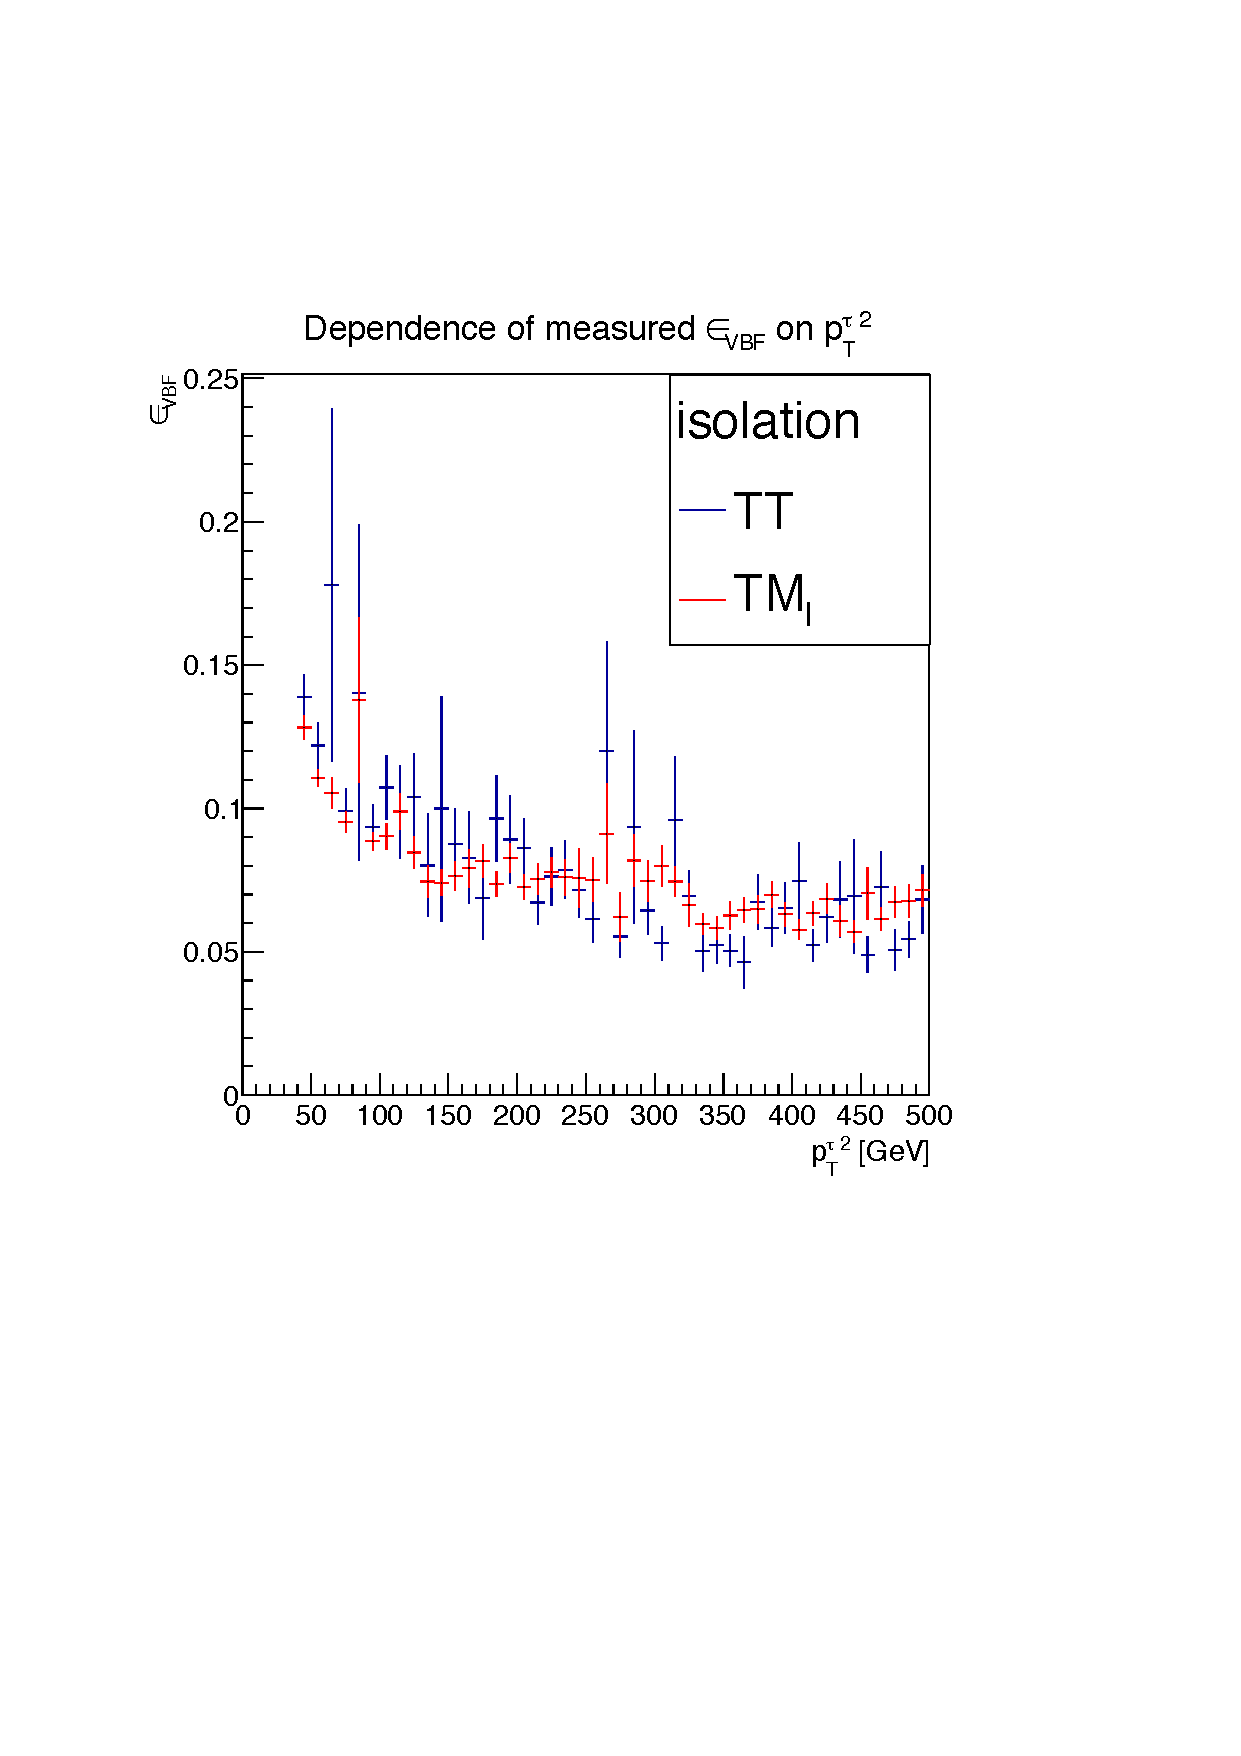
\includegraphics[width=0.5\textwidth]{analysis/pics/vbeff_vs_tauiso.pdf}
	\caption{Distribution of $\epsilon^{VBF}$ against the second to leading \hadtau momentum in case of two \hadtau passing a tight (TT) or loose ($\text{TM}_{\text{I}}$) isolation requirement. It can be observed $\epsilon^{VBF}$ decreases before stabilizing at high momenta \cite{bib:phdthesis:denis}.}
	\label{dihad:fig:vbeff_vs_tauiso}
\end{figure}

An additional stability study is performed by considering the deviation of the weighted arithmetic mean of $\epsilon^{VBF}$ with respect to \met as shown in \autoref{dihad:fig:vbeff_vs_met}. A quadratic divergence, caused by the impact of higher jet energy resolution widths over the forward sections of the detector, is observed. An additional systematic uncertainty is derived in order to take this effect into account.

\begin{figure}[!h]
	\centering
	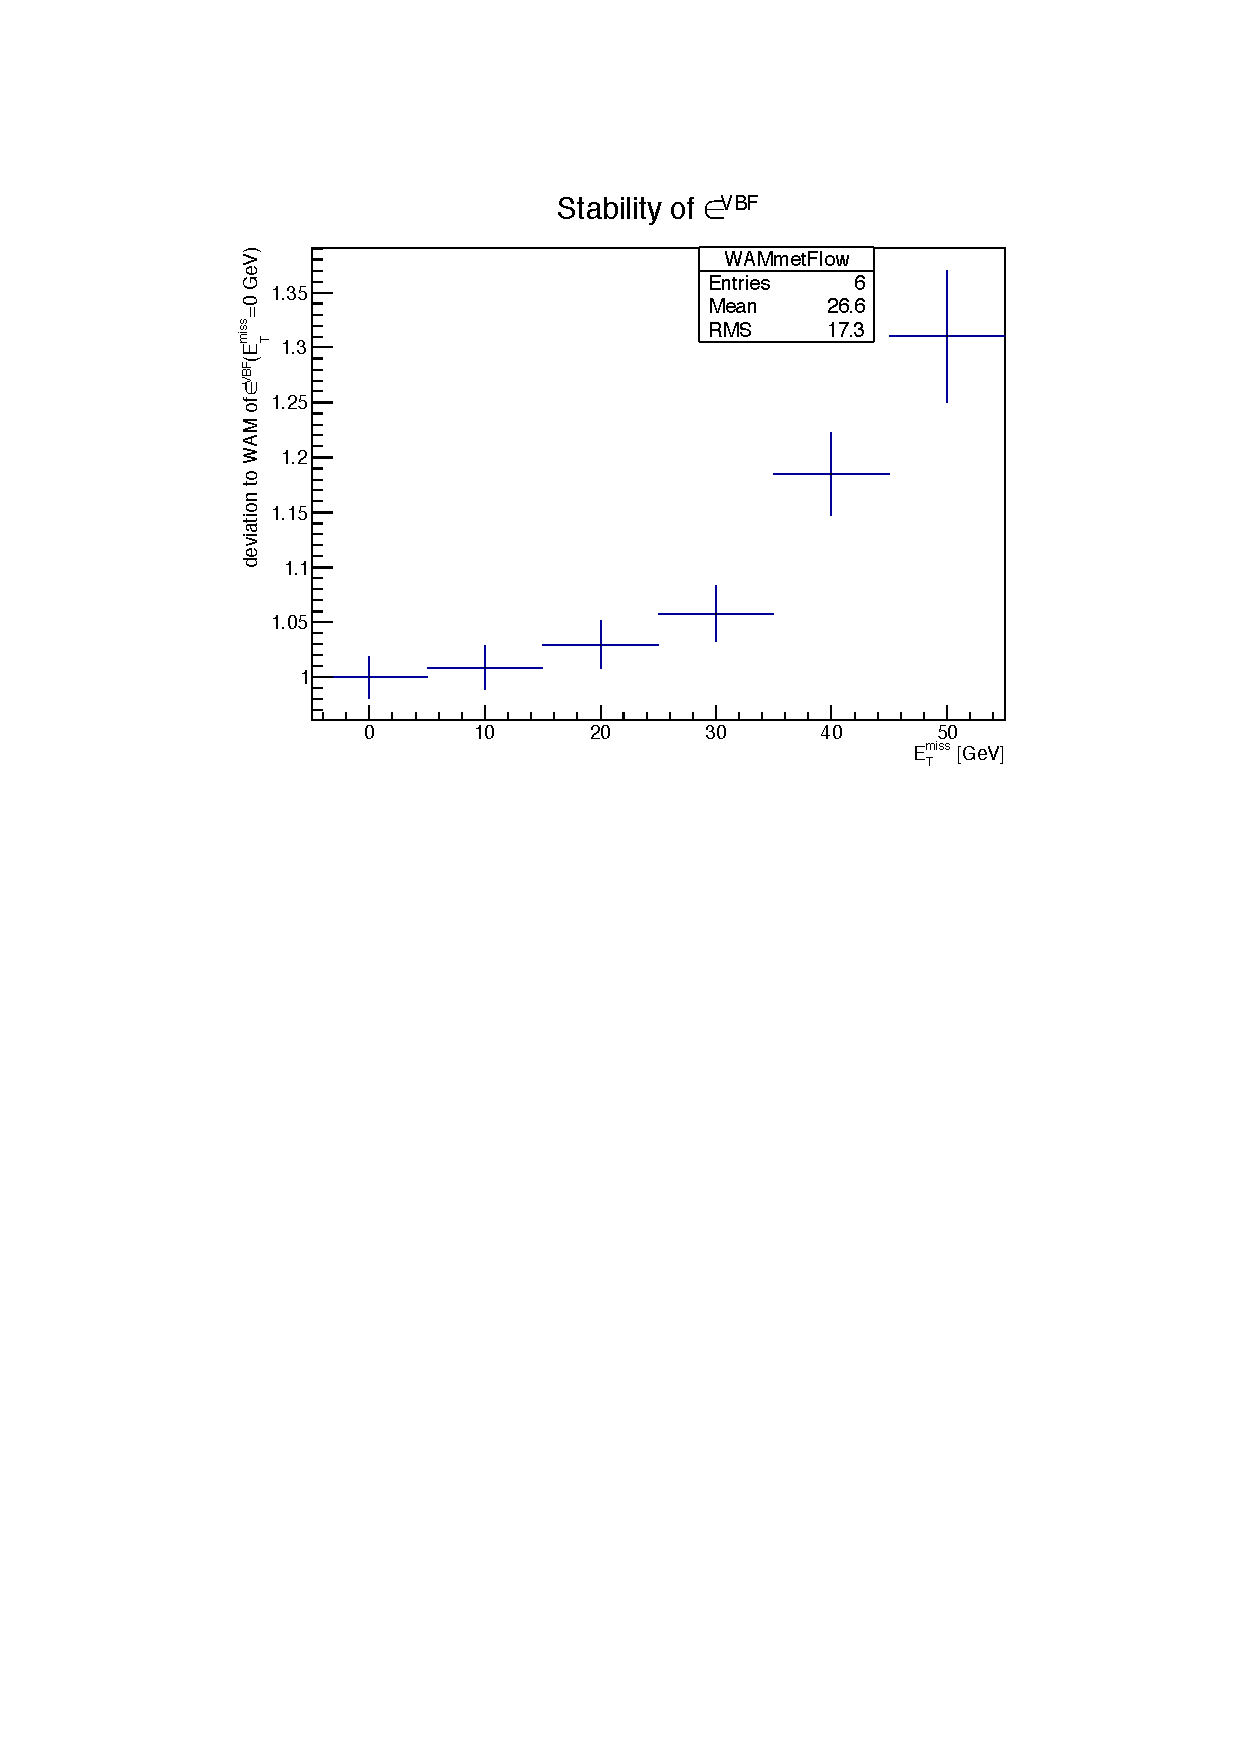
\includegraphics[width=0.5\textwidth]{analysis/pics/vbeff_vs_met.pdf}
	\caption{Deviation of the weighted arithmetic mean (WAM) of the VBF efficiency of all control region ratios with respect to \met. A slight quadratic divergence is observed for $\met > 30\gev$ \cite{bib:phdthesis:denis}.}
	\label{dihad:fig:vbeff_vs_met}
\end{figure}
 
To summarize, two systematic uncertainties are taken into account in this study:

\begin{enumerate}
	\item Stability of $\epsilon^{VBF}$ with respect to \hadtau-isolation: Maximum relative difference to weighted arithmetic mean at \met 30\gev. This amounts to $+17.26\%$ and  $-7.58\%$ relative uncertainty.
	\item Stability of $\epsilon^{VBF}$ with respect to \met-requirement: Relative difference to $\epsilon^{VBF}$ within uncertainties of weighted arithmetic mean at no selection on \met. This amounts to $+8.30\%$ relative uncertainty on the upper edge and $+3.26\%$ on the lower edge.
\end{enumerate}


\clearpage

\section{Signal samples systematic uncertanties}
\label{sec:systematics}

The following systematics have been considered while estimating the signal samples contribution in signal region:

\begin{itemize}
	\item \textbf{Parton Distribution Functions (PDF):} The systematic effect due to imprecise knowledge of the parton distribution functions is determined by comparing CTEQ6.6L \cite{Nadolsky:2008zw}, MSTW2008nnlo \cite{Martin:2009iq}, and NNPDF20 PDF \cite{Ubiali:2008uk} with the default PDF and variations within the family of parametrization. The maximal deviation from the central value is used as the overall systematic uncertainty due to PDFs. We obtain a value of 16\% on the cross section uncertainty and 23\% on the signal acceptance.
	
	\item \textbf{Initial State Radiation (ISR) and Final State Radiation (FSR):} The systematic effect due to imprecise modeling of initial and final state radiation is determined by re-weighting events to account for effects such as missing a terms in the soft-collinear approach \cite{Nanava:2003cg} and missing NLO terms in the parton shower approach \cite{Miu:1998ju}. We obtain uncertainties of 0.9\% and 1.2\% for ISR and FSR respectively.
	
	\item \textbf{Luminosity:} We consider a 2.6\% uncertainty on the measured luminosity \cite{CMS:2012rua}.
	
	\item \textbf{Trigger, Reconstruction, and Selection:}  An overall uncertainty is applied for the trigger uncertainties determined on the correction factors described in \cite{bib:AN-12-321} and which are measured using tag-and-probe methods. We consider 6.8\% uncertainty per hadronic tau leg \cite{CMS:2011msa}. Scale factors for $\tau_{h}$ identification are taken from the tau POG and obtained using a fit of data in a Z$\to\tau\tau$ enhanced region and fixing the cross section to that measured using ee/$\mu\mu$. We consider a 100\% correlation among the 2 tau legs, therefore we consider 13.6\% uncertainty on the signal acceptance.
	
	\item \textbf{$b$-Tagging Efficiency:} We consider a 30\% uncertainty on the mis-tag rate as measured by the b-tagging POG \cite{CMS:2011cra}. For the case of our signal, the systematic uncertainty on the requirement of 0 jets mis-tagged as b-jets is determined by propagating the 30\% uncertainty on the mis-tag rate through the following equation (which represents the signal efficiency for requiring 0 jets mis-tagged as b-Jets):
	
	\begin{equation}\label{eq:nttbar}
	\epsilon^{\textrm{NBtag} < 1} = 1 - \sum_{n=1} P(n) \cdot \sum_{m=1}^{n} C(n,m) \cdot f^{m} \cdot (1-f)^{n-m}
	\end{equation}
	
	where $P(n)$ is the probability to obtain $n$ additional jets (non-tau and non-lepton) in the event, $C(n,m)$ the combinatorial of $n$ $choose$ $m$, and $f$ the mis-tag rate. The probability to obtain at least one additional jet in the event is much less than 1\%. Therefore, based on the above equation, the mis-tag rate and uncertainty, and the probability to obtain at least one additional jet we calculate a negligible systematic effect on our signal due to the mis-tag rate.
	
	\item \textbf{Tau Energy Scale:} We consider the effect of the 3\% tau energy scale uncertainty measured by the tau POG on the signal acceptance. The tau 4-momentum is scaled by a factor of $k=1.03$ ($p_{scaled} = k \cdot p_{default}$) and variables are recalculated using $p_{scaled}$. We find that by using $p_{scaled}$ calculated with a factor of $k=\pm 1.03$, the signal acceptance fluctuates by 4\%. Therefore, we assign a 4\% systematic on the signal acceptance due to tau energy scale.
	\item \textbf{Jet Energy Scale:}  The uncertainty on jet energy correction (JEC) is the result of a factorized approach on $Anti­-k_{t}$ jets with $R=0.5$ clustered from Particle Flow (PF) candidates. For MC samples JEC is divided in different steps that take into account several levels of correction. The fist step consist in a single level of corrections (L1) which estimates the $p_{t}$ offset in bins of $\eta$ and $N_{PV}$ for AK5PF jets. The second step, known as MC-Truth Corrections, consists in two level of corrections (L2 and L3) converging into an $\eta$ , $p_{t}$ ­dependent scaling factor fully derived from MC after applying L1­ corrections. The last step takes into account an L5 correction and uncertainties for individual flavors and predefined mixtures inside the reconstructed jets. We assign a 2\% systematic on the signal acceptance due to jet energy scale.
	\item \textbf{Jet Energy Resolution:}  The measured jet transverse momentum is never equal to the energy of the original particle due to e.g. a limited detector resolution. This effect is quantified by the jet transverse momentum response R which is defined as $R = p_{T} / p_{T}^{particle}$  where $p_{T}$ denotes the transverse momentum of the jet measured at detector level and $p_{T}^{particle}$ is the transverse momentum of the original particle-level jet. The average response $\langle R \rangle$ is referred to as jet energy scale and calibrated such that $\langle R \rangle = 1$ for fixed $p_{T}^{particle}$. The response usually depends on the jet momenta as well as on the pseudorapidity. This is expected since the quality of the jet measurement is directly related to the detector sub-components and the energy of the particles originating e.g. from the track-reconstruction efficiency or the individual amount of detector material. The core of the response is caused by the intrinsic resolution of the various sub-detector components and the precision of the jet clustering algorithms. The response tails are mainly caused by severe jet-mismeasurements. These can be e.g. detector effects like shower leakage or detector noise. Finally, the relative jet transverse momentum resolution is defined as the width of the response distribution corresponding to the gaussian part and hence is a function of $p_{T}$ and $\eta$ as well as the total response. One possibility to measure the resolution of the jet transverse momenta in data as well as in simulated events is to utilize the dijet asymmetry A. For events with at least two jets it is defined as:
	
	\begin{equation}
	A = \frac{p_{T,1} - p_{T,2}}{p_{T,1} + p_{T,2}}
	\end{equation}
	
	For a sufficient number of events the asymmetry is approximately normally distributed and its standard deviation is $\sigma_{A}$. In an ideal dijet topology the two jets are exactly balanced at particle level which leads to an important relation between the width of the asymmetry $\sigma_{A}$ and the jet-$p_{T}$ resolution $\sigma(p_{T})$:
	
	\begin{equation}
	\frac{\sigma(p_{T})}{\langle p_{T} \rangle} = \sqrt{2} \sigma_{A}
	\end{equation}
	
	Using the latest JER uncertainty collection from \texttt{Summer13\_\-V5\_DATA\_\-Uncertainty\-Sources\_\-AK5PFchs.txt} assign a 4\% systematic on the signal acceptance due to jet energy resolution. 
	
	\item \textbf{MET:} The uncertainty on MET for our signal process is driven by the jet energy scale (non-tau jets) (JES), light lepton energy/momentum scale (LES), and unclustered energy (UCE). The systematic effect from MET due to TES, JES and LES is included in the JES, TES, LES systematic uncertainties described above. We find that a 10\% uncertainty on the unclustered energy results in at most a 0.5\% fluctuation on the signal acceptance.
\end{itemize}

\begin{table}[h]
	\centering{
		\begin{tabular}{| l | c | c |}
			\hline\hline
			Source            & Initial uncertainty & Signal uncertainty\\
			\hline
			PDF               & ---                            & 23\%                       \\
			ISR/FSR           & ---                             & 1\%              \\
			Luminosity        & 2.6\%                           & 2.6\%                      \\
			Trigger, ID, Selection & 6.8\%                            & 16\%                       \\
			Tau Energy Scale  & --                             & 4\%                        \\
			b-Jet ID          & 30\%                            & 1\%                        \\
			JES               & 2\% - 10 \%                            & 2\%                      \\
			JER              & 5\% - 25 \%                            & 4\%                      \\
			MET               & 10\%                           & 0.5\%  \\
			\hline\hline                  
		\end{tabular}
	}
	\caption{Summary of systematic uncertainties}
	\label{table:Uncertainties}
\end{table}

\autoref{table:Uncertainties} summarizes all the relevant uncertainties that has been considered for the generated signal samples. 

\clearpage

\section{Results}
\label{section:results}

Following the procedure described in \autoref{sec:bgestimation}, $\epsilon^{QCD}_{VBF}$ is calculated for both the di-\hadtau sign channels: opposite-sign (OS) and like-sign (LS). All the uncertainties described in \autoref{sec:bgestimation} and \autoref{dihad:subsec:stability} have been taken into account and have been properly propagated. The weighted average mean coming from the two different measurements gives the following final result:

\begin{equation}
\epsilon^{QCD}_{VBF} = 0.067\pm0.0046(stat.)^{-0.00038(MC)+0.0117(\tau iso)+0.0056(MET)}_{+0.00022(MC)-0.0051(\tau iso)+0.0022(MET)}
\label{eq:vbfefflsresult}
\end{equation}

Using this result as input for \autoref{eq:qcdbgpred} gives the final QCD background prediction in signal region:

\begin{equation}
N^{QCD}_{SR} = 7.59\pm0.92(stat.)^{-0.42(MC)+1.34(\tau iso)+0.20(MET)}_{+0.35(MC)-0.58(\tau iso)-0.20(MET)}
\label{dihad:eq:QCDbgpredCorrectResult}
\end{equation}

The like-sign signal region consist of events satisfying the criteria shown in section \ref{sec:eventselection} with the di-$\tau$ charge requirement. \autoref{table:SReventcount} shows the contributions in the signal region from all MC samples and data. As described in section \ref{dihad:subsec:eventweight}, the QCD and W+jet  background contribution have been "diced" and accordingly reweighted. 

QCD is the dominant background and its data-driven prediction shown in \autoref{dihad:eq:QCDbgpredCorrectResult} is fully compatible within statistical and systematic uncertainty with the simulation-driven results shown in \autoref{table:SReventcount}. 

\met and \mjj distribution in the signal region (SR) for data and Monte Carlo are shown in \autoref{fig:LS_SR_h_met_dijetinvariantmass_log}.

\begin{table}[ht]
	\centering{
		
		%   \tabcolsep=0.05cm
		\begin{tabular}{| l | c |}
			\hline\hline
			Sample     &Events (SR)      \\ [0.5ex] \hline
			Data &$ 9 $     \\
			Drell-Yan &$ 0.037\pm0.015$      \\
			VV &$ 0.11\pm0.065$     \\
			W+Jets &$ 0.53\pm0.04$        \\
			Single t &$ 0.036\pm0.0066$    \\
			TTbar &$ 0.11\pm0.012$    \\
			Higgs &$ 0.0005\pm7.2e-05$     \\
			QCD Prediction &$ 7.59\pm0.92(stat.)^{+1.38}_{-0.72}(syst.)$    \\
			\hline
			Total nonQCD MC &$ 0.83\pm0.079(stat.)\pm0.41(syst.)$    \\
			\hline\hline
		\end{tabular}
	}
	\caption{\label{table:SReventcount}Number of events for data and all Monte Carlo contribution in the signal region. The QCD prediction has been corrected for the unidirectional MET-bias described in section \ref{dihad:subsec:stability} for the combination of the systematic errors.}
	% is used to refer this table in the text
\end{table}

\begin{figure}[tbh!]
	\centering
	\begin{tabular}{cc}
		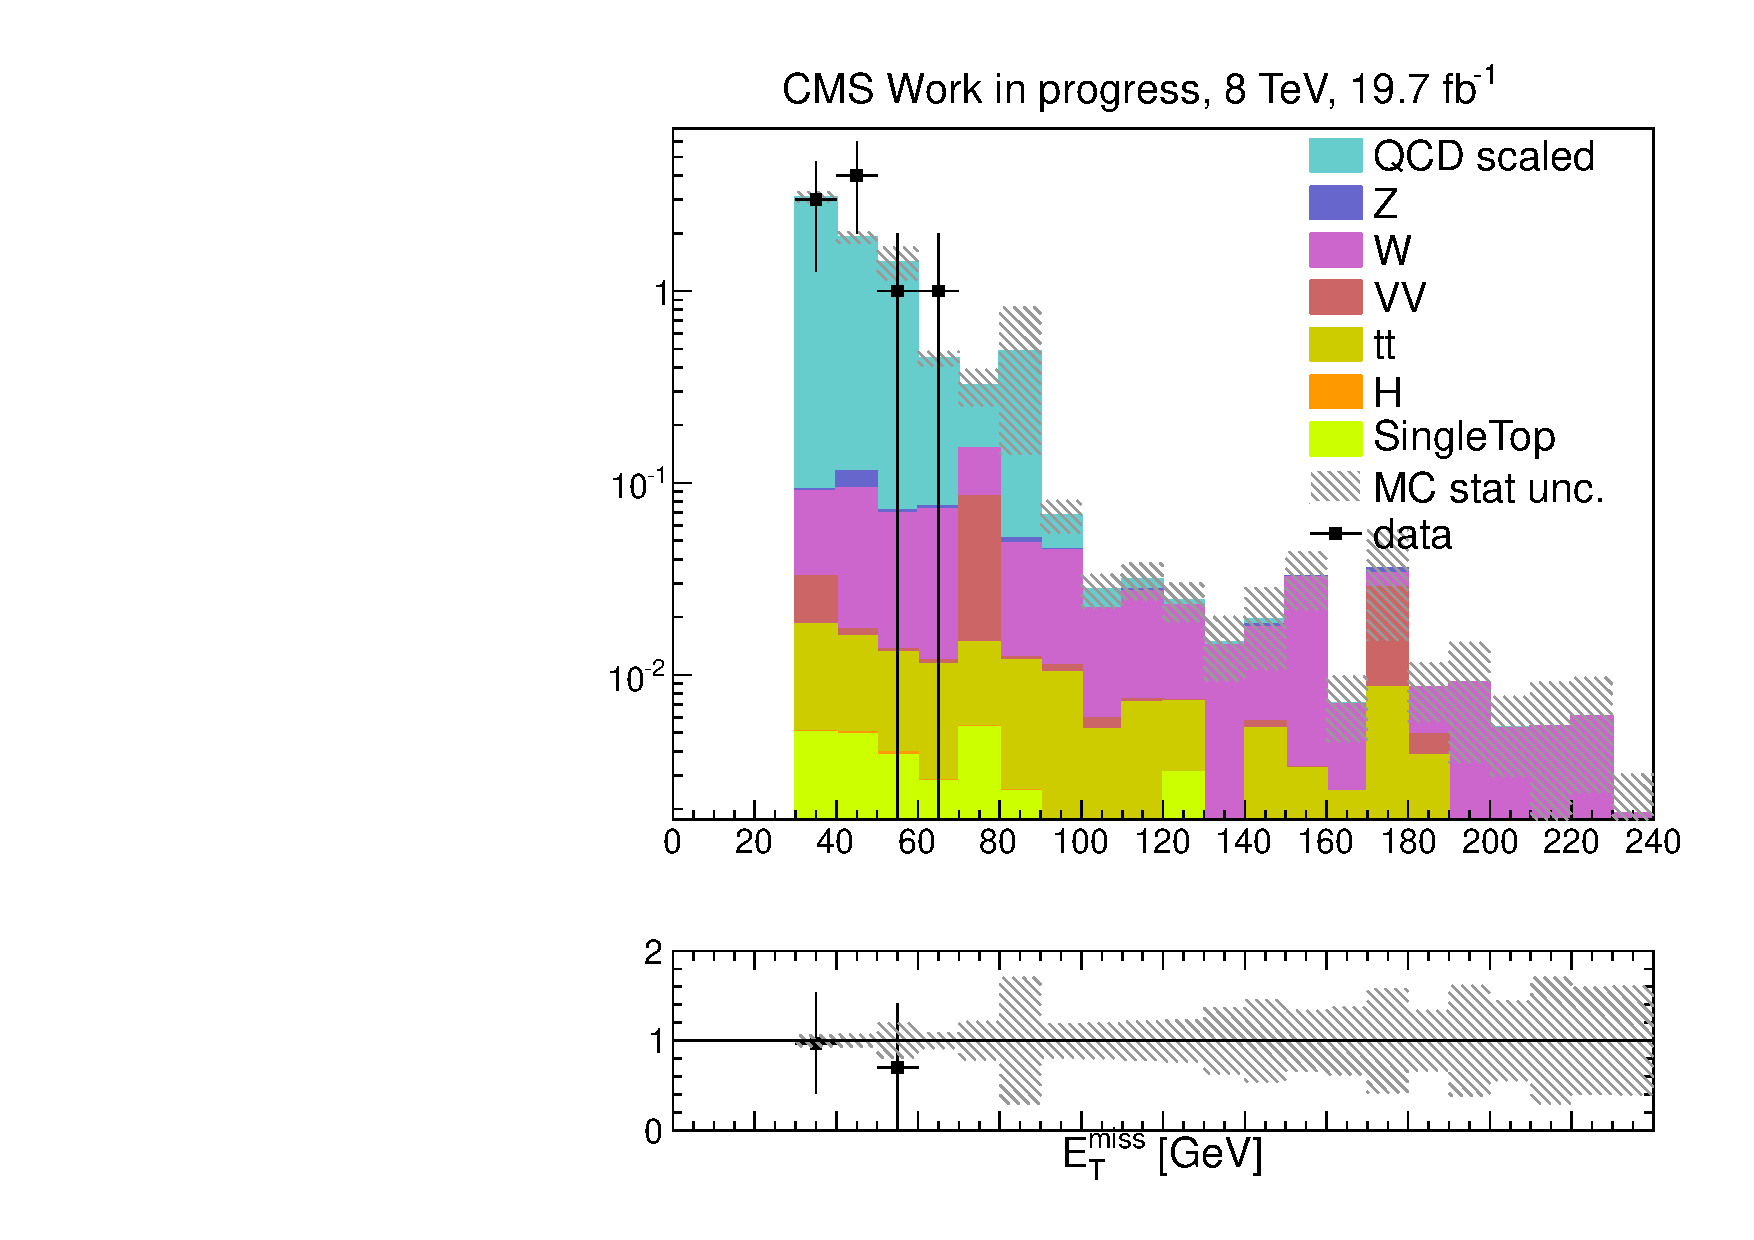
\includegraphics[width=0.40\textwidth]{PLOTS/diTauHadLSQCDPlots/UnblindedUpdate/LS_SR/LS_SignalRegion/h_met_log.pdf}
		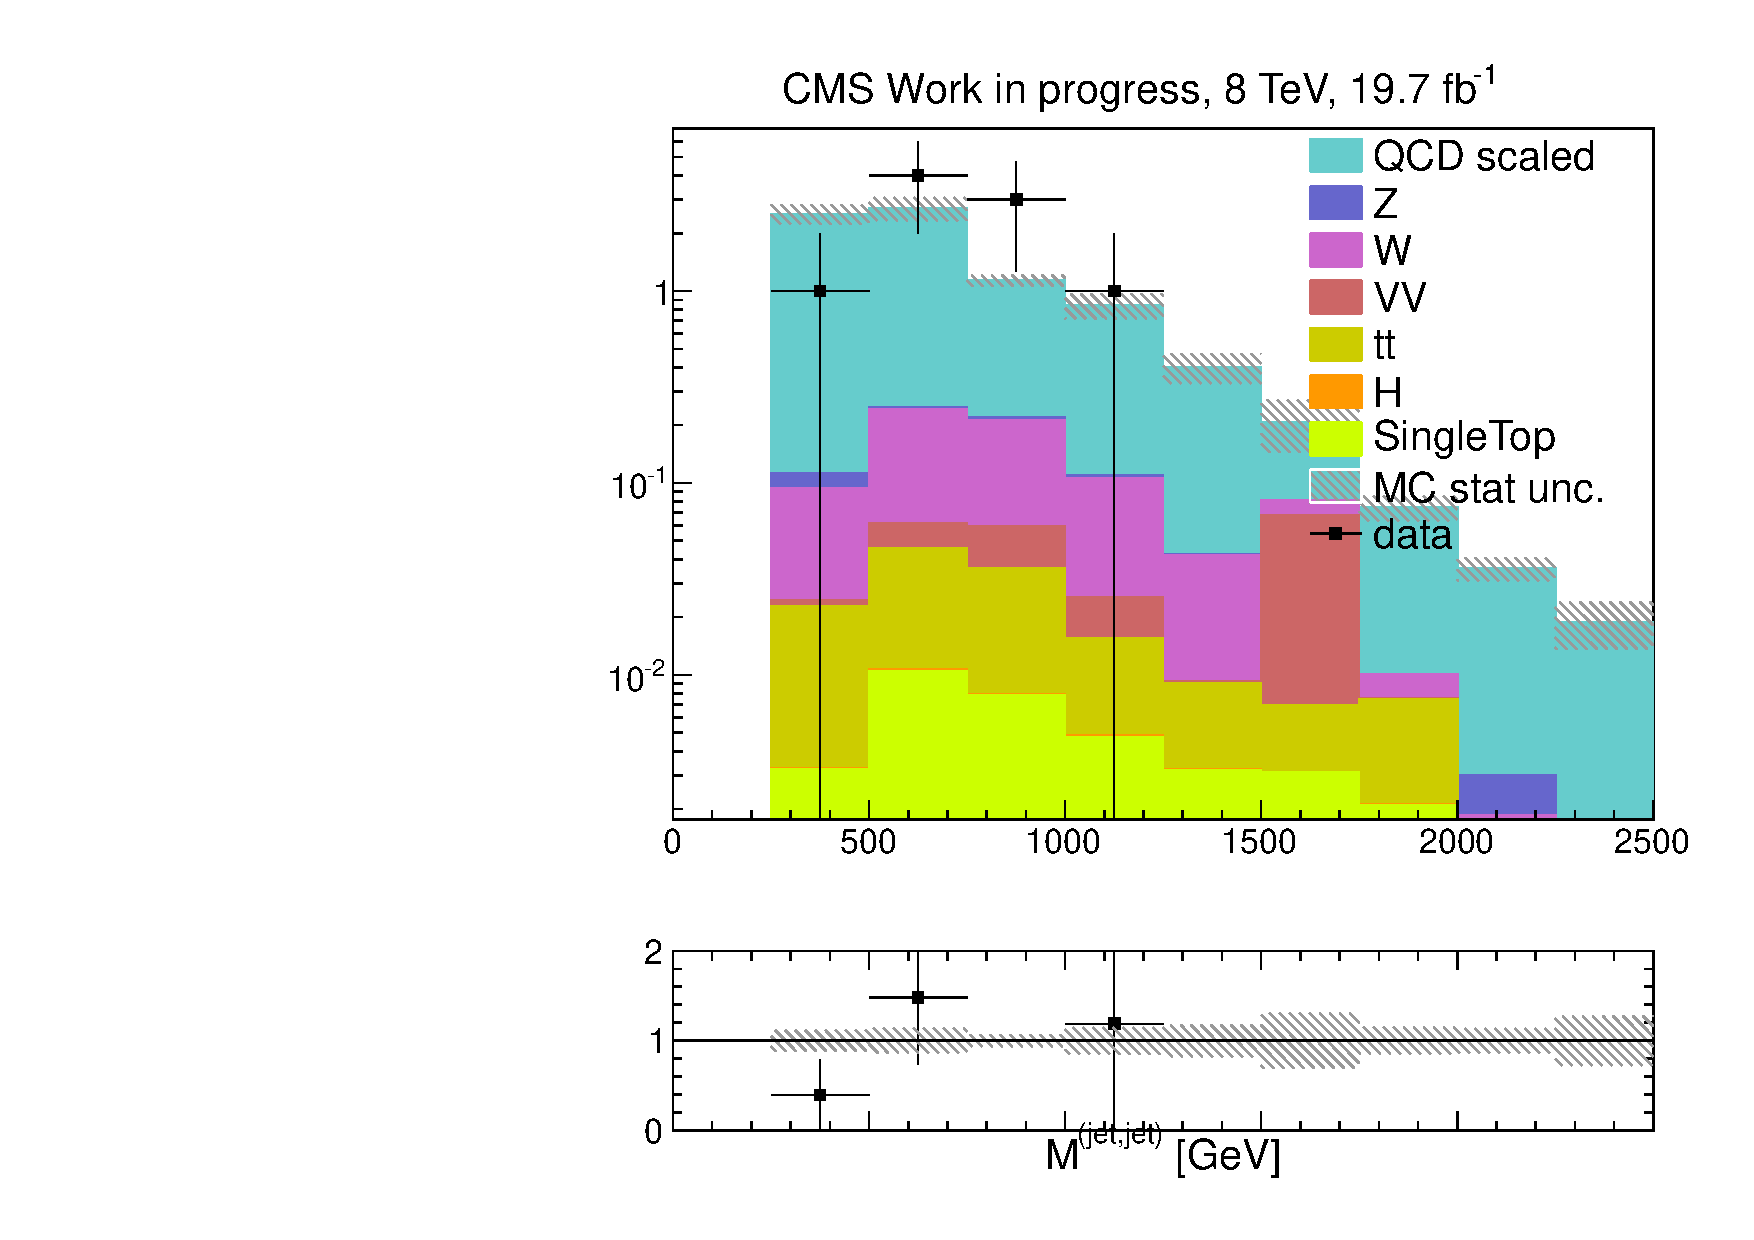
\includegraphics[width=0.40\textwidth]{PLOTS/diTauHadLSQCDPlots/UnblindedUpdate/LS_SR/LS_SignalRegion/h_dijetinvariantmass_log.pdf}
	\end{tabular}
	\caption{(a) \met and (b)$M_{jj}$ distributions in signal region for Data and all MC samples}
	\label{fig:LS_SR_h_met_dijetinvariantmass_log}
\end{figure} 

A combination of the opposite and like-sign signal yields coming from all the different search channels is shown on \autoref{fig::mjj_combined} as \mjj distribution \cite{Khachatryan:2015kxa}.

\begin{figure}[!h]
	\centering
	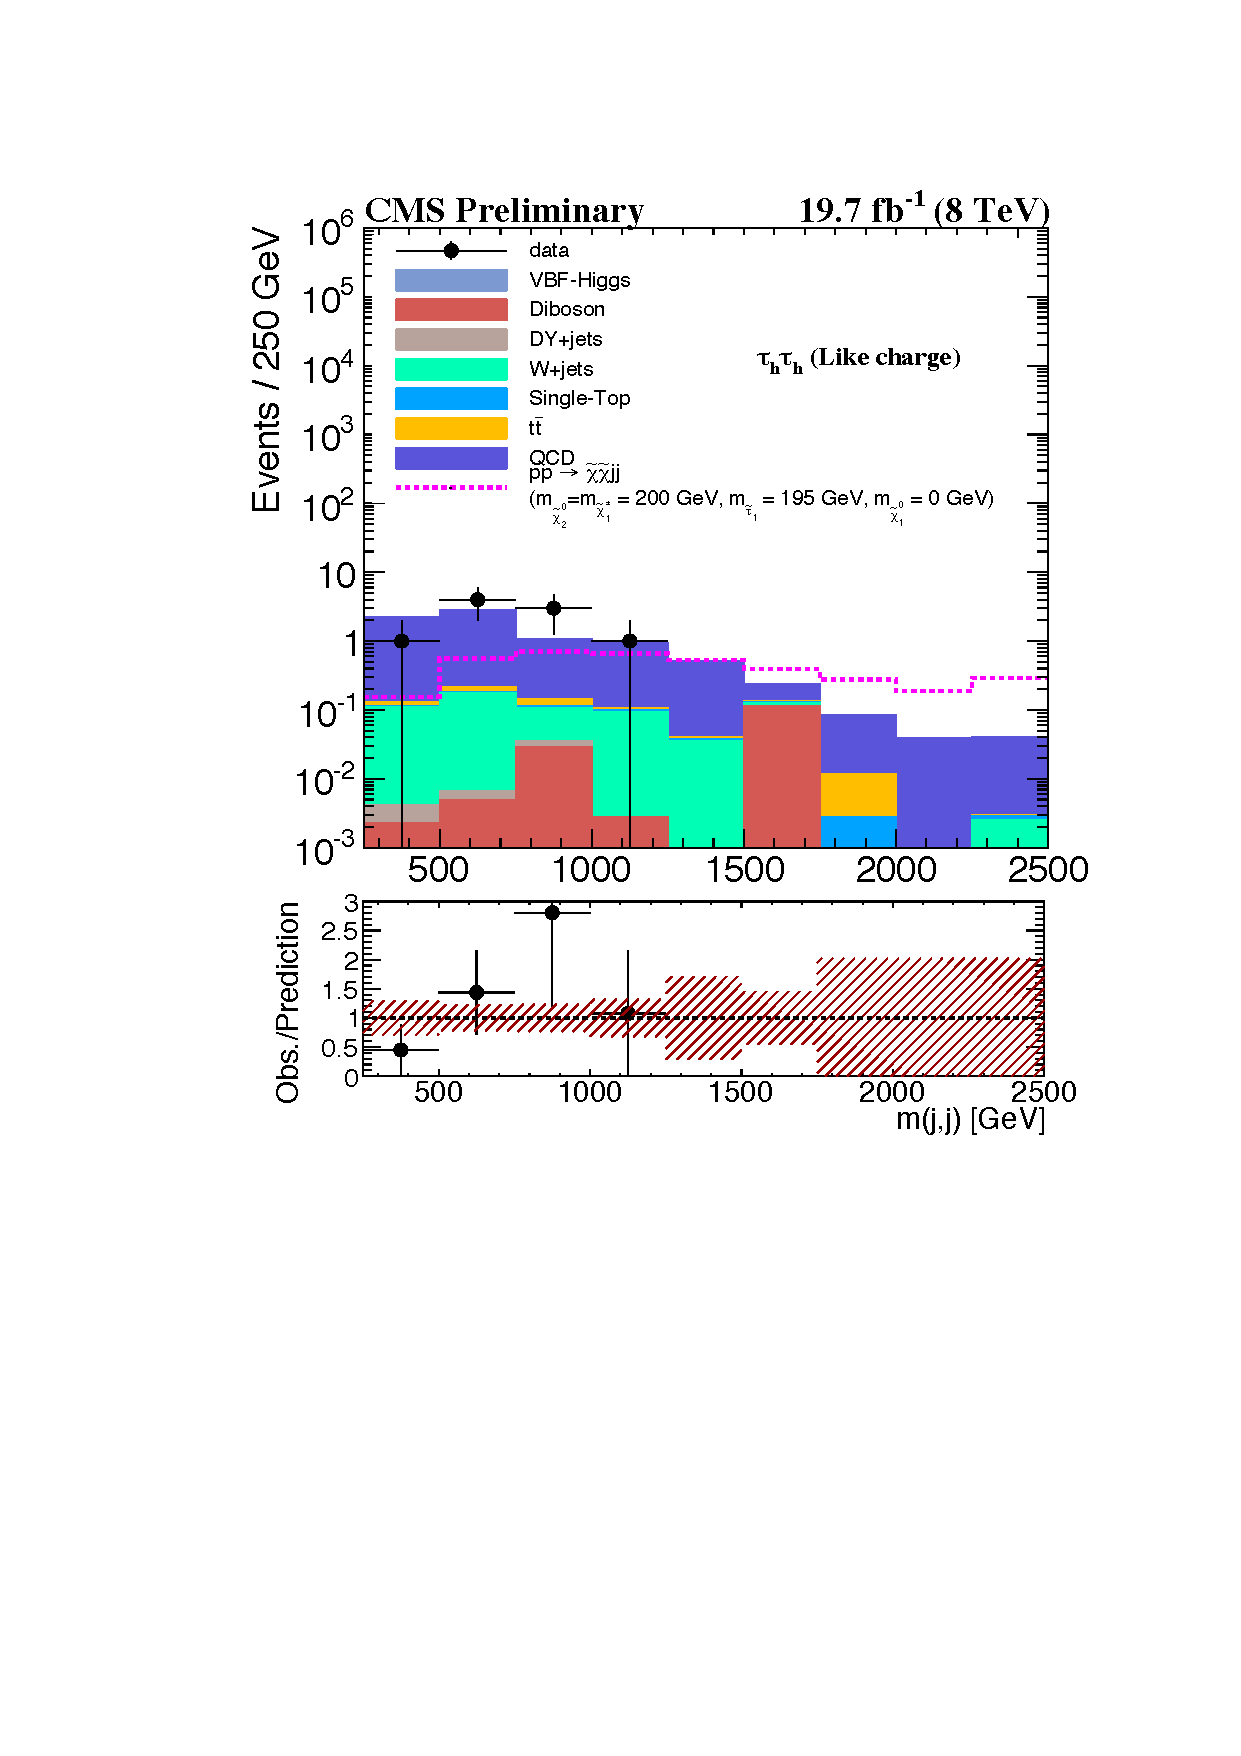
\includegraphics[width=0.5\textwidth]{analysis/pics/mjj_combined.pdf}
	\caption{The final yields of the like sign di-\hadtau channel. No excess above standard model expectation is observed \cite{Khachatryan:2015kxa}.}
	\label{fig::mjj_combined}
\end{figure}

\section{Exclusion limits on chargino/neutralino masses}

Upper limits at $95\%$ on the cross sections as function of $m_{\tilde{\chi}_{2}^{0}}=m_{\tilde{\chi}_{1}^{\pm}}$ are set for like-sign and opposite channel. The results are presented using models with a fixed mass for the LSP $m_{\tilde{\chi}_{1}^{0}} = 0\gev$, a $\tilde{\chi}_{1}^{\pm}$ mass between $100 \leq m_{\tilde{\chi}_{1}^{\pm}} \leq 300\gev$ and a $\tilde{\tau}$ mass of $m_{\tilde{\tau}} = 0.95 m_{\tilde{\chi}_{1}^{\pm}}$ .

\begin{figure}
	\begin{center}
		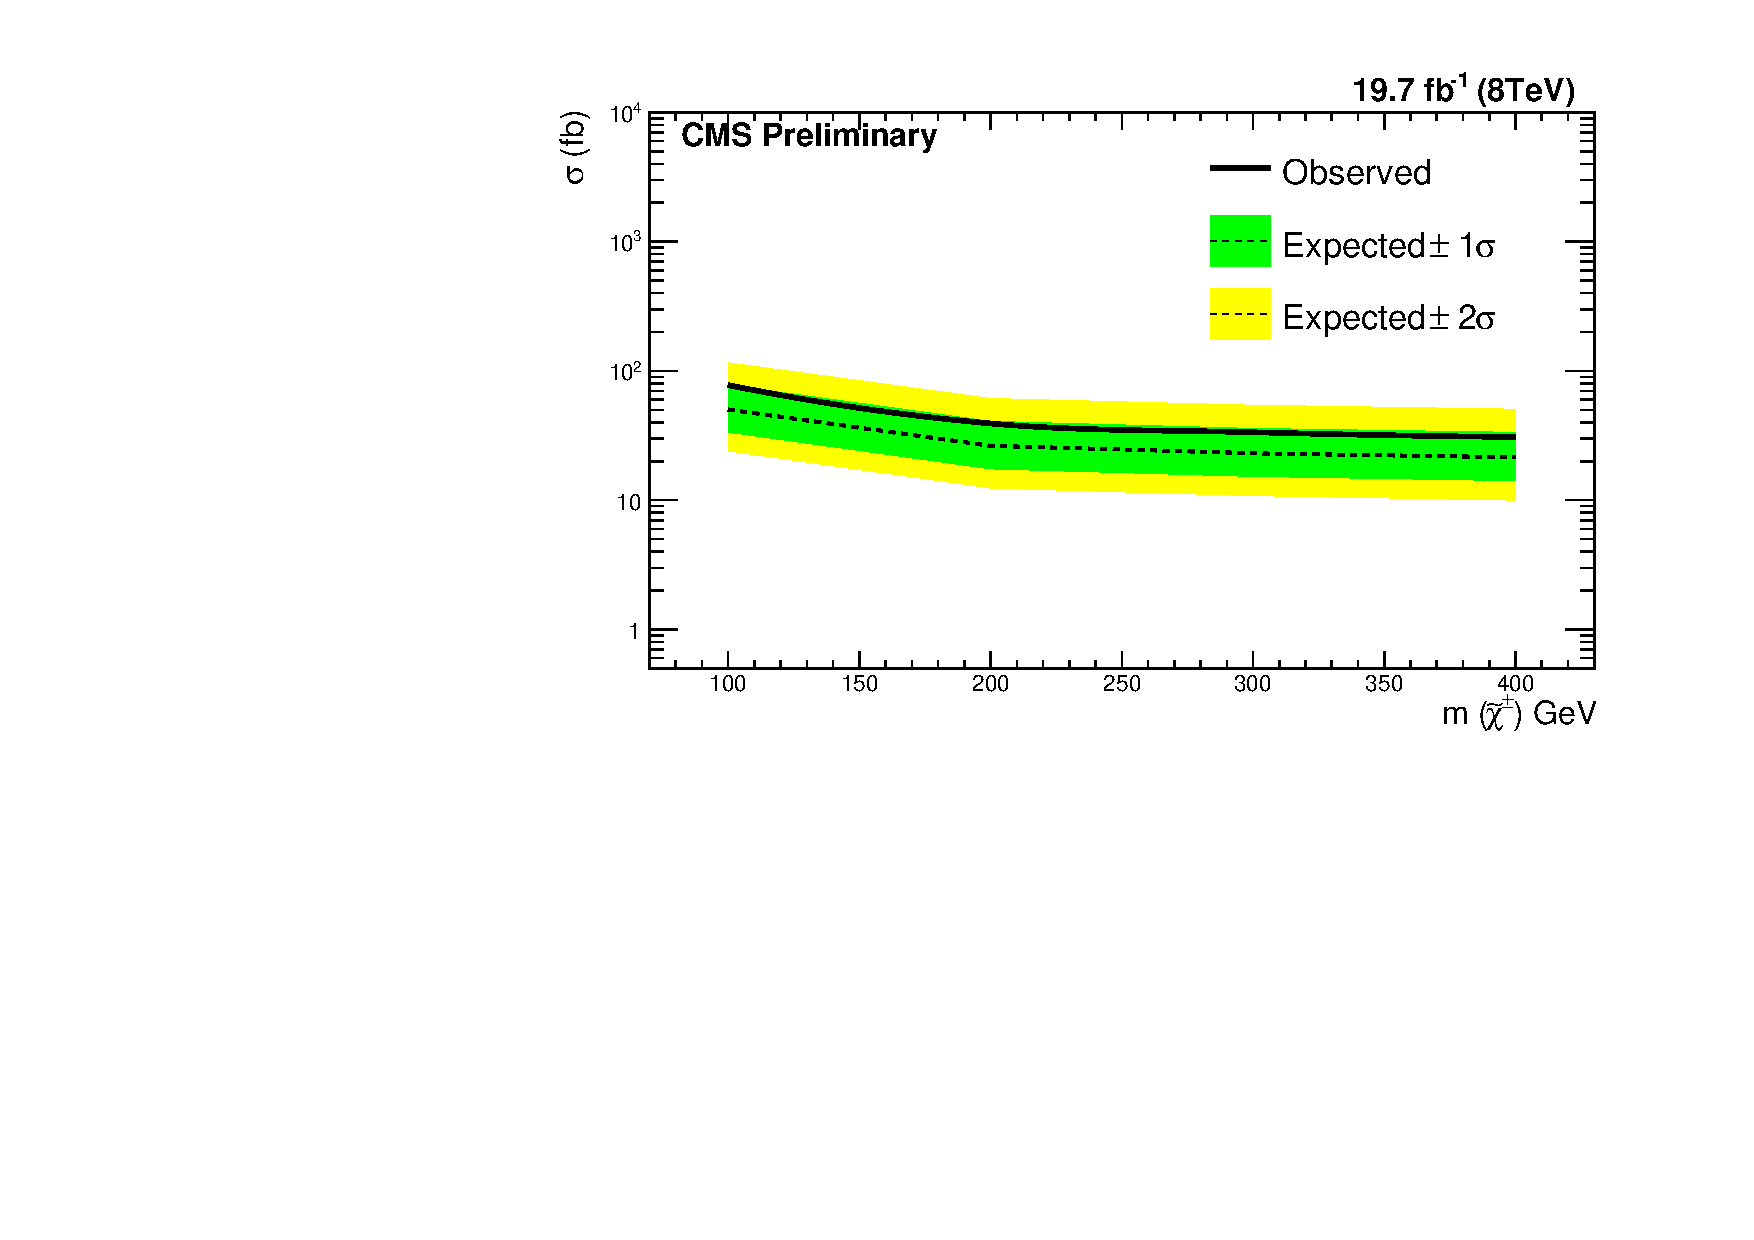
\includegraphics[angle=0,width=.48\textwidth, height=0.35\textheight]{PLOTS/Limit_VBF_diTau_OS.pdf}
		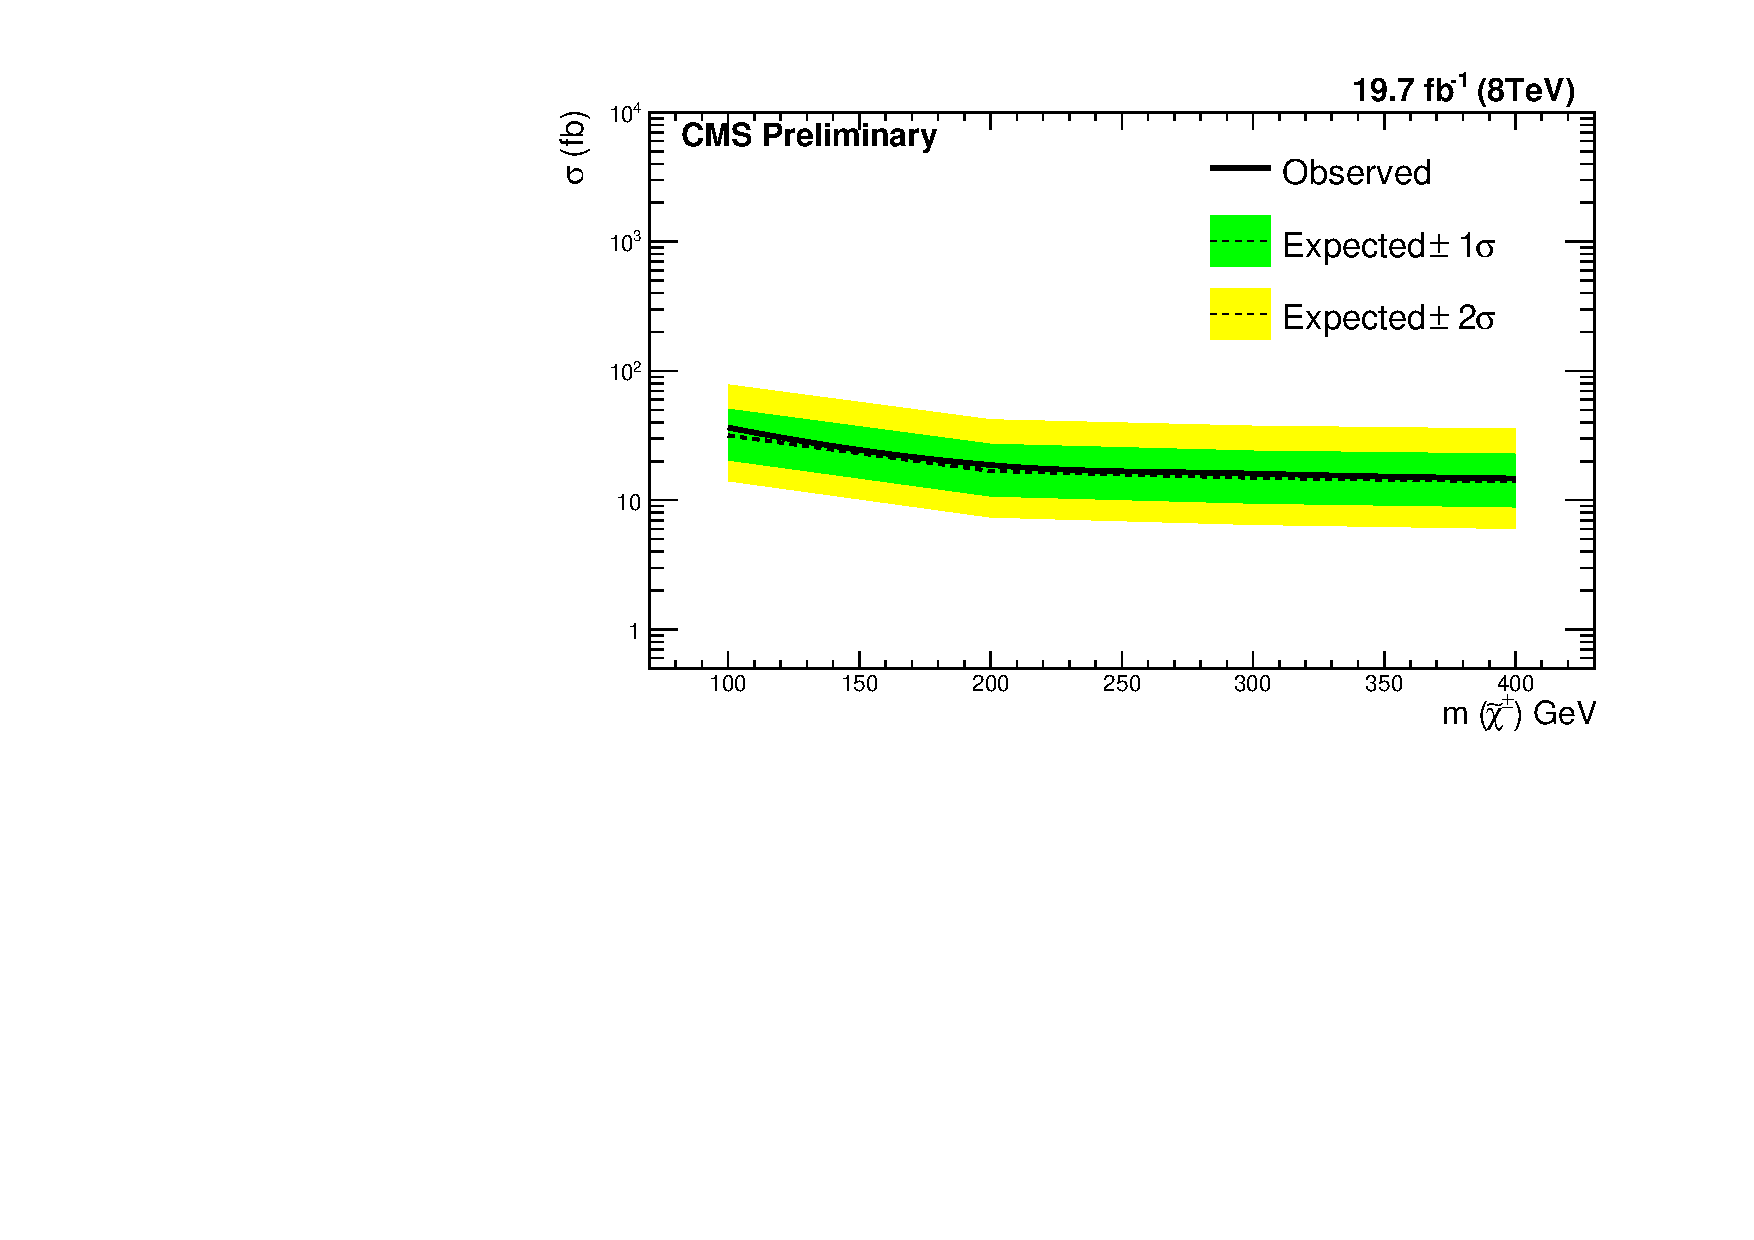
\includegraphics[angle=0,width=.48\textwidth, height=0.35\textheight]{PLOTS/Limit_VBF_diTau_LS.pdf}
		\caption{Upper limit at the 95\% CL on the cross-section as a function of 
			$m_{\tilde{\chi}_{2}^{0}}=m_{\tilde{\chi}_{1}^{\pm}}$ for the (a) OS 
			$\tau_{h}\tau_{h} j_{f} j_{f}$, (b) LS $\tau_{h}\tau_{h} j_{f} j_{f}$
			final states. The bands represent the one and two standard deviations obtained from the background-only hypothesis.}
		\label{fig:LimitsOSLS}
	\end{center}
\end{figure}

\begin{figure}
	\begin{center}
		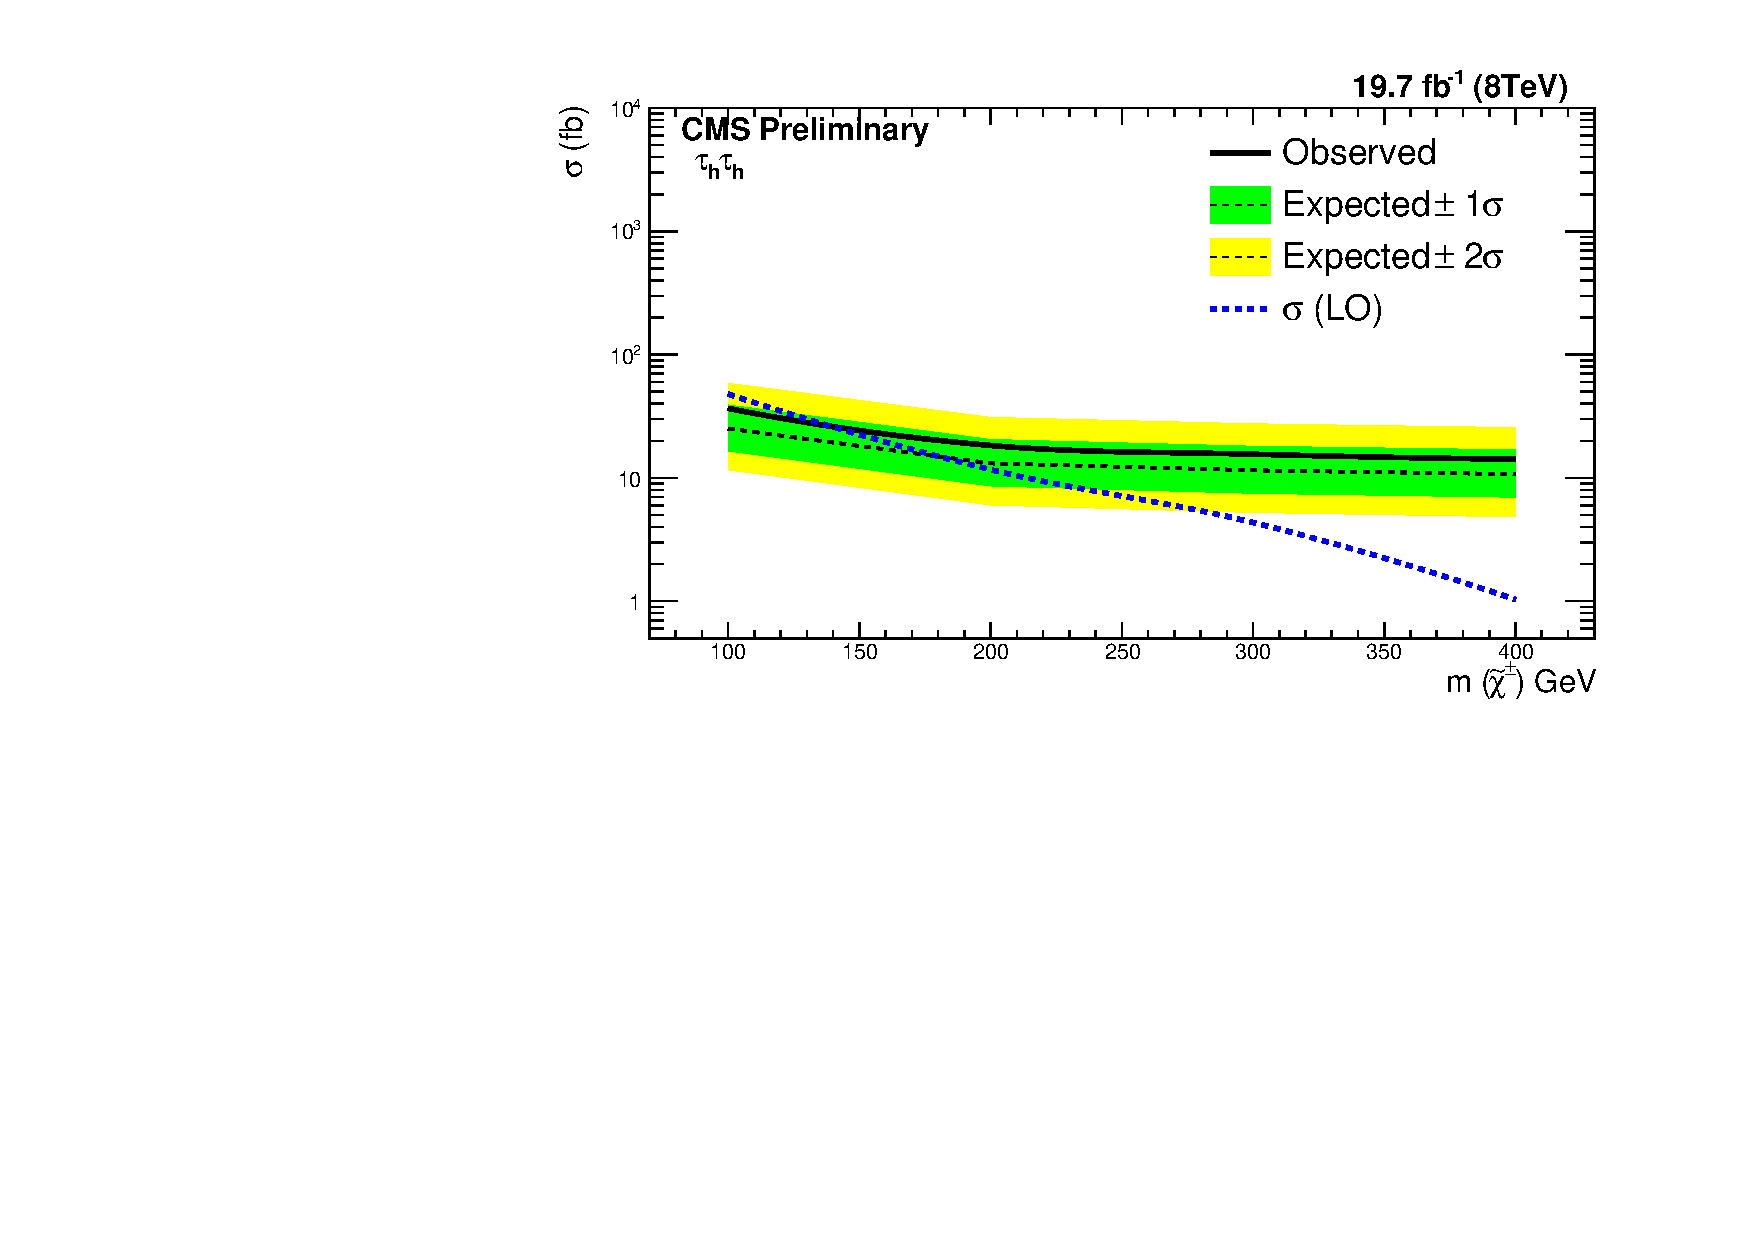
\includegraphics[angle=0,scale=0.75]{PLOTS/Limit_VBF_diTau_combined.pdf}
		\caption{Upper limit at the 95\% CL on the cross-section as a function of 
			$m_{\tilde{\chi}_{2}^{0}}=m_{\tilde{\chi}_{1}^{\pm}}$ for the combination of OS and LS $\tau_{h}\tau_{h} j_{f} j_{f}$
			final states. The bands represent the one and two standard deviations obtained from the background-only hypothesis.}
		\label{fig:LimitsCombination}
	\end{center}
\end{figure}

 \autoref{fig:LimitsOSLS}  shows the upper limit at the 95\% CL on the cross-section for opposite and like-sign channel. A combination of the two channels is shown on \autoref{fig:LimitsCombination}. The upper expected limit on $m_{\tilde{\chi}}$ corresponds to the point where the expected limit crosses the theoretical line and is set for  $\tilde{\chi}_{1}^{\pm} /\tilde{\chi}_{2}^{0} $ with masses of 180\gev. The upper observed limit on $m_{\tilde{\chi}}$ corresponds to the point where the observed limit crosses the theoretical line. In the model considered, $\tilde{\chi}_{1}^{\pm} /\tilde{\chi}_{2}^{0} $ with masses below 140\gev are excluded.
 
The limit results coming from opposite and like-sign $\tau_{h}\tau_{h} j_{f} j_{f}$ final states are combined with other 6 channels documented on \cite{Khachatryan:2015kxa} for the final upper limit.
